\documentclass{sigchi}


% EXAMPLE BEGIN -- HOW TO OVERRIDE THE DEFAULT COPYRIGHT STRIP -- (July 22, 2013 - Paul Baumann)
\toappear{Permission to make digital or hard copies of all or part of this work for personal or classroom use is
granted without fee provided that copies are not made or distributed for profit or commercial advantage and that 
copies bear this notice and the full citation on the first page. Copyrights for components of this work owned by 
others than ACM must be honored. Abstracting with credit is permitted. To copy otherwise, or republish, to 
post on servers or to redistribute to lists, requires prior specific permission and/or a fee. 
Request permissions from permissions@acm.org. \\
{\emph{ISWC'15}}, September 7--11, 2015,Osaka, Japan. \\
Copyright \copyright~2014 ACM ISBN/14/04...\$15.00. \\
DOI string from ACM form confirmation}
% EXAMPLE END -- HOW TO OVERRIDE THE DEFAULT COPYRIGHT STRIP -- (July 22, 2013 - Paul Baumann)




% Arabic page numbers for submission. 
% Remove this line to eliminate page numbers for the camera ready copy
% \pagenumbering{arabic}




% Load basic packages
\usepackage{balance}  % to better equalize the last page
\usepackage{graphics} % for EPS, load graphicx instead
\usepackage{times}    % comment if you want LaTeX's default font
\usepackage{url}      % llt: nicely formatted URLs

% llt: Define a global style for URLs, rather that the default one
\makeatletter
\def\url@leostyle{%
  \@ifundefined{selectfont}{\def\UrlFont{\sf}}{\def\UrlFont{\small\bf\ttfamily}}}
\makeatother
\urlstyle{leo}

% To make various LaTeX processors do the right thing with page size.
\def\pprw{8.5in}
\def\pprh{11in}
\special{papersize=\pprw,\pprh}
\setlength{\paperwidth}{\pprw}
\setlength{\paperheight}{\pprh}
\setlength{\pdfpagewidth}{\pprw}
\setlength{\pdfpageheight}{\pprh}

% Make sure hyperref comes last of your loaded packages, 
% to give it a fighting chance of not being over-written, 
% since its job is to redefine many LaTeX commands.
\usepackage[pdftex]{hyperref}
\hypersetup{
pdftitle={SIGCHI Conference Proceedings Format},
pdfauthor={LaTeX},
pdfkeywords={SIGCHI, proceedings, archival format},
bookmarksnumbered,
pdfstartview={FitH},
colorlinks,
citecolor=black,
filecolor=black,
linkcolor=black,
urlcolor=black,
breaklinks=true,
}

% create a shortcut to typeset table headings
\newcommand\tabhead[1]{\small\textbf{#1}}


%%%%%%%%%%%%%%%%%%%%%%%%%%%%%%
%ADDITIONAL PACKAGES
\usepackage{booktabs}
\usepackage[table]{xcolor}% http://ctan.org/pkg/xcolor


% End of preamble. Here it comes the document.
\begin{document}

\title{Skills Assesment for Salsa Dancers \\
Through the Phase Space Representation}

\numberofauthors{3}
\author{
  \alignauthor author 1\\
    \affaddr{Affiliation}\\
    \affaddr{Address}\\
    \email{e-mail address}\\
    \affaddr{Optional phone number}
  \alignauthor author 2\\ %Chris Baber\\
    \affaddr{Affiliation}\\
    \affaddr{Address}\\
    \email{e-mail address}\\
    \affaddr{Optional phone number}    
  \alignauthor author 3\\ %Neil Cooke\\
    \affaddr{Affiliation}\\
    \affaddr{Address}\\
    \email{e-mail address}\\
    \affaddr{Optional phone number}
}

\maketitle

\begin{abstract}
This paper presents a description of the use of time-delay embedding, using Taken's Theorem, 
to analyse data from Inertial Measurement Units mounted on people performing Salsa dance steps.  
The aim of the work is to understand how dexterity can be described in terms of the consistency 
and variability of human activity. To this end, approaches which rely on the definition of 
discrete events or states might not capture dexterity in the same manner. 
The paper shows the application of the approach to expert, intermediate and novice dancers, 
and how these different dancers can be distinguished from the patterns of data the approach produces. 
The paper concludes with a discussion of the potential uses of time-delay embedding for 
Human Activity Recognition using data from wearable sensors.


\end{abstract}

\keywords{Activity Recognition; Skill Assesment; Nonlinar Dynamics; Time-series analysis;
}


\category{I.5.4.}{Pattern Recognition}{Applications}


\section{Introduction}

The use of data from wearable sensors to identify human activity is a staple of wearable computer research.
%Bulling et al. \cite{Bulling2014}. 
A core challenge arises from the need to partition these data into segments 
which can be used to label repetitions of discrete events which correlate with specific actions. 
Such an approach draws on signal processing techniques developed to work in the frequency domain and can, 
through stochastic processes, be used to recognise sequences of events.  As Hammerla et al. \cite{Hammerla2011}
note ``[t]herefore information about what subjects are doing is readily available, rendering activity 
segmentation a straight-forward follow up task''. 
In previous work, we have shown that it is possible to distinguish between skill levels for jewellery 
students performing simple tasks, using sensors embedded in their tools \cite{RefXXX}.
This study used Principal Components Analysis of the data from intertial sensors to define 
clusters of variables that formed classes which could be used to distinguish between novice, intermediate 
and expert performance.  In their study of the dynamics of tennis serves,  Ahmadi et al. \cite{Ahmadi2010}, 
show that use of marker-based motion-capture or inertial measurement units (accelerometer and gyroscope) 
on the person, can be equally effective in identifying the level of skill shown by people making serves 
in tennis.  They showed that skill level corresponds to peak values in velocity for shoulder rotation, 
wrist flexion and upper arm internal rotation prior to a tennis serve. These studies suggest that the objective 
classification of skill can be made from data acquired from on-body sensors. 
Such an approach accords well with the view of expertise as the definition of a motor schema (see below). 
However, dexterity can also be explained as the optimal control of specific parameters and, for this perspective, 
recognition of sequences of events might not be sufficient. 

Identifying how \textit{well} an action is performed is more challenging. 
When it comes to studying skilled or dextrous performance, recognition of sequences of events 
might not be sufficient. 
There are two reasons for this:
(i) The raw data from sensors, in their original, canonical basis, contain no information regarding the structure of
the activity. Variability in these data could arise from at least three sources:
inherent properties of the activity itself;
discrepances of expertise between expert and beginners, or between different steps;
inherent noise in the sensors.
(ii) Dexterity in human activity is seldom matter of performing events 
faster or even of sequencing the events in the same manner as the novice. 
% Rather, the expert segues actions 
% into smooth sequences which, through their overlapping and intertwining, become difficult for event-based 
% approaches. An alternative is to apply time-series techniques to such data. The focus of this paper is on 
% the use of a specific time-series technique to explore a specific aspect of dextrous performance. 
% However, the approach can be easily applied to other data and domains. Before explaining the approach, 
% the paper begins with a short discussion of dexterity in human performance.


% An alternative is to apply time-series techniques to such data.

The focus of this paper is on the use of a Takens' Theorem for the phase space representation 
to explore a specific aspect of dextrous performance. 
However, the approach can be easily applied to other data and domains. 
Before explaining the approach, the paper begins with a short discussion of dexterity in human performance. 


\section{DEXTERITY IN HUMAN PERFORMANCE AND HUMAN ACTIVITY RECOGNITION}
Studies of skilled psychomotor performance indicate that expertise is not simply a matter of performing actions 
in a more consistent manner than novices \cite{Kelso2014}. Often the expert is able to produce different but 
contextually appropriate actions in a manner that the novice is unable to perform. This highlights a paradox 
in human motor control: in order to act consistently, people need to produce stable patterns of movement 
which can be repeated efficiently, but these movements also need to exhibit sufficient variability to cope 
with changes in contextual demand. 
Biomechanics research explains this control of movement in two broad approaches: 
a common approach is to assume that a movement is specified in a hierarchy of commands, 
with a high-level description of a goal defined in terms of location of end-point of that movement, 
from which it is possible to calculate optimal paths. 
For these approaches, consistency is 
explained through the definition of ``motor schema'' which specifies the neural commands required to enervate 
the musculoskeletal system to perform a specific action. In such a system, variability in movement arises 
from noise and interference in the translation of motor command to the performance of the movement. 
This means that variability is seen as something which needs to be either ignored or dismissed. 
For Human Activity Recognition, the motor schema view could lead to the assumption that it is beneficial 
to either filter out such noise or to define averaged patterns which capture the underlying consistency 
in movement and recognise activity against these patterns. 

% An alternative approach sees variability in human movement as defined by the originating system. 
Yamamoto and Gohara \cite{Yamamoto2000} defined dexterity as ``$\ldots$ the capacity of goal-directed movement 
to adapt itself to changes in the external environment$\ldots$''  An action involves the coordination of muscles and 
joints in an efficient manner. This raises the ''degrees of freedom``, or ''motor equivalence``, 
problem \cite{Bernstein1967}. 
The motor equivalence problem notes that each joint in the human body has several degrees of freedom in 
the postural angles that it can adopt, and that combining several joint angles in a given movement can 
result in a great many alternative postures, particularly when actions are performed dynamically. 
While people might appear to be making consistent motions in repetitive actions, there is sufficient 
variability to make it difficult to define a single solution to the motor equivalence problem. 
The challenge here is to reconstruct the originating system in such a way to 
compute the minimal parameters which are being optimised in the performance of the movement. 
From this perspective, dexterity, 
or expert performance, could arise from the use of specific parameters in the control of movement and 
the assumption is that experts seek to optimise different parameters to novices. 
 

Previous work on the application of dynamical systems approaches to the study of human activity sought to 
reconcile Bernsteins  \cite{Bernstein1967} 'degrees of freedom' problem with the mathematics 
of dynamical systems \cite{Kugler1982}.
% An influential early research paradigm was devleoped by Haken, Kelso and Bunz \cite{Haken1985}
% In this work, participants performed a very simple task (alternate tapping of index fingers in time to a metronome) 
% and it was demonstrated that, once the speed exceeds a certain threshold, the two fingers stop moving out of 
% phase and move in phase. This shift is abrupt and indicates a change in attractor state of a dynamical 
% system which is seeking to optimise specific order parameters  \cite{Beek1995, RefXXX}.
Viewing human motor control in terms of 
dynamical systems allows researchers to consider how dexterity capitalises on the inherent ''noisiness`` of the human 
movement system. This approach has been particularly fruitful in the field of skill in sports \cite{Davids2003}
and we believe that it offers an interesting perspective for activity recognition. 
Applying this assumption to Human Activity Recognition, the goal would be to identify the parameters that are being 
optimised in a data stream produced when activity is performed, rather than identifying 
discrete events within that data stream. 
 

\section{RECOGNISING DEXTERITY IN DANCE }
As Miura et al. \cite{Miura2015} point out ''$\ldots$ how the human motor system produces dance movements in still 
poorly understood.`` A key issue concerns the manner in which experienced dancers solve the degrees of freedom 
problem in the face of changing contextual demands.  Miura et al. \cite{Miura2013} measured muscle activation 
using electromyography (EMG) collected from muscles in the lower limb, for a task requiring participants to 
bounce up and down in time to a metronome beat.  They demonstrated that experienced dancers show much better 
precision in synchronizing movements to beat than non-dancers, i.e., dancers maintained much lower standard 
deviation in temporal deviation against the beat than non-dancers. This result is consistent with work which 
shows that, compared with inexperienced- or non-dancers, trained ballet dancers exhibit superior postural 
stability \cite{Crotts1996} %(Crotts et al., 1996) 
, and show superior ability in position matching of upper limbs \cite{Ramsay2001}.%(Ramsey and Riddoch, 2001).  

Capturing dance activity through sensors has tended to rely on motion capture 
\cite{Alexiadis2014} %(Alexiadis and Daras, 2014) 
or sensors mounted on the person \cite{Lynch2005} %(Lynch et al., 2005) 
or in their shoes \cite{Paradiso1997} %(Paradiso and Hu, 1997) 
or from their smartphones  \cite{Wei2014}. %(Wei et al., 2014).  
Much of this work has been concerned with using the dancers’ motion to work with 
multimedia presentations that augment and complement the dance \cite{Griffith1998, Park2006}
%(Grifith and Fernstrom, 1998; Park et al., 2006) 
or as interfacing to a game \cite{Chu2012} %(Chu et al., 2012) 
or commercial games, such as Dance Dance Revolution.  
While the range of sensing technology used in these papers is diverse and the result of the activity 
recognition is varied, it is fair to say that few of the papers have considered 
variability or dexterity in how well dance is performed. 
In their work, Aristidou et al. \cite{Aristidou2014} %(2014) 
have considered the manner in which dance steps conform to a set of defined 
templates that describe steps in terms of three-dimensional rotation (described using quaternions).  
The implication is that a goodness-of-fit can be ascertained to determine how well a dancer performs a step, 
and how any deviation from ‘good’ can be modified through practice. 


For this paper, we are interested in the question of how time-series techniques can provide insight into 
the dexterity of dancers. To this end, we consider the performance of a set of steps from Salsa dance and 
compare untrained, inexperienced or non-dancers in one cohort with experienced dancers in another. 
Before explaining how data were collected, the next section outlines the approach to time-series analysis,
phase space representation used in this paper. 
It should be noted that dynamical systems research offers a range of techniques for the study of human activity 
(see \cite{Guastello2011} for an overview of alternative techniques). 
However, this paper focuses on a specific technique which utilises Taken's Theorem.






\section{PHASE SPACE REPRESENTATION OF THE TIME SERIES DATA}
In this work we follow the notation employed in \cite{Uzal2011}.
The purpose of the Takens's Theorem, also known as time-delay embedding, 
is to reconstruct a $D-$dimensional manifold \textbf{M} $s(t)$ of an unknown dynamical 
system from time series $x(t)$ of that system.
Thus, we assume that the signal we are observing has been produced by some time-varying system 
(rather than been generated entirely at random).  
The assumption that the source of the signal exhibits systematic variation then leads to the further 
assumption that this signal should, over some time period, exhibit a repeated pattern or a meta-stability.  
What we do not know is what this time period might be or what this pattern might look like.  
Thus, time-delay embedding assumes that the time series is a sequence $x(t)=h(s(t))$, 
where $h: M \rightarrow \mathbb{R}^D$ is a measurement function on the unknown dynamical system, 
being $x(t)$ observable.
The time delay reconstruction in $m$ dimensions with time delay $\tau$ is defined as:
$\overline{x}(t) = (x(t), x(t-\tau),...,x(t-(m-1)\tau))$ which defines a map
$\varPhi: M \rightarrow \mathbb{R}^m$ such that $\overline{x}(t) = \varPhi(s)$.
$\varPsi: \mathbb{R}^m \rightarrow \mathbb{R}^n$ is a further transformation that
is considered as a more general transformation (Figure \ref{fig:takens_theorem}).
In order to decompose the resulting data set we apply
% in which for the current work we are applying the 
Principal Component Analyis (PCA).
\begin{figure}[!htb]
\centering    
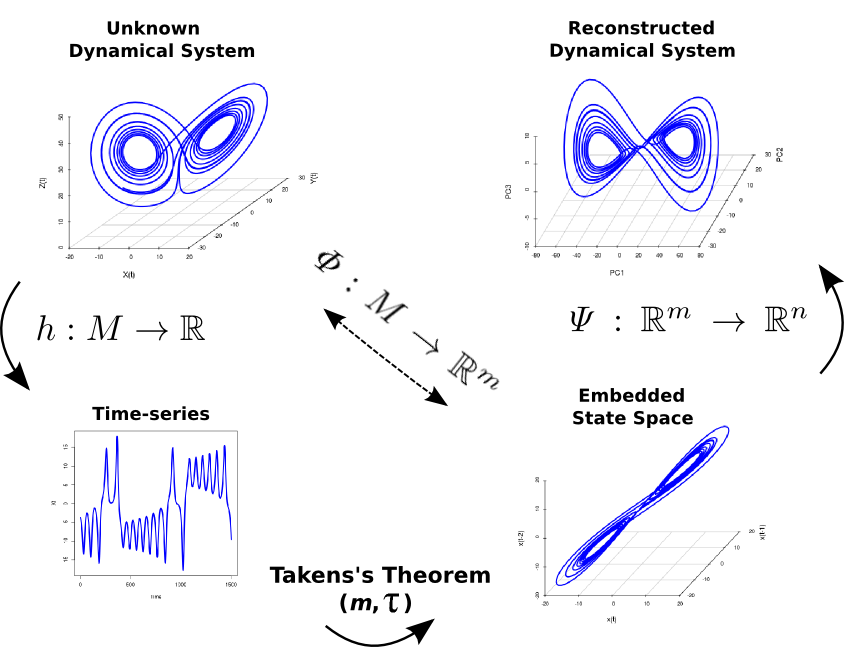
\includegraphics[width=0.45\textwidth]{takens_theorem_v4}
\caption[PA]{The reconstruction problem}
\label{fig:takens_theorem}
\end{figure}
Therefore, our approach is based on the collection of raw data from an 
Inertial Measurement Unit (IMU) for triaxial data 
for accelerometer (ACC), gyroscope (GYR) and magnetometer(MAG) sensors. 
Then, for instance, the time-series $a_x$ with a length of 
$N$ samples is used to obtain the Time-delay embedded matrix, 
$\boldsymbol{E} a_{x}$, with $m$ rows and $N-(m-1)\tau$ columns. 
Finally, the PCA algorithm is applied so as to obtain eigenvalues 
($\lambda_1,\ldots,\lambda_m$), eigenvectors ($v_1,\ldots,v_m$) and principal components 
($PC_1,\ldots,PC_m$) (Figure \ref{fig:raw_takens_pca}).
\begin{figure*}[!ht]
\centering    
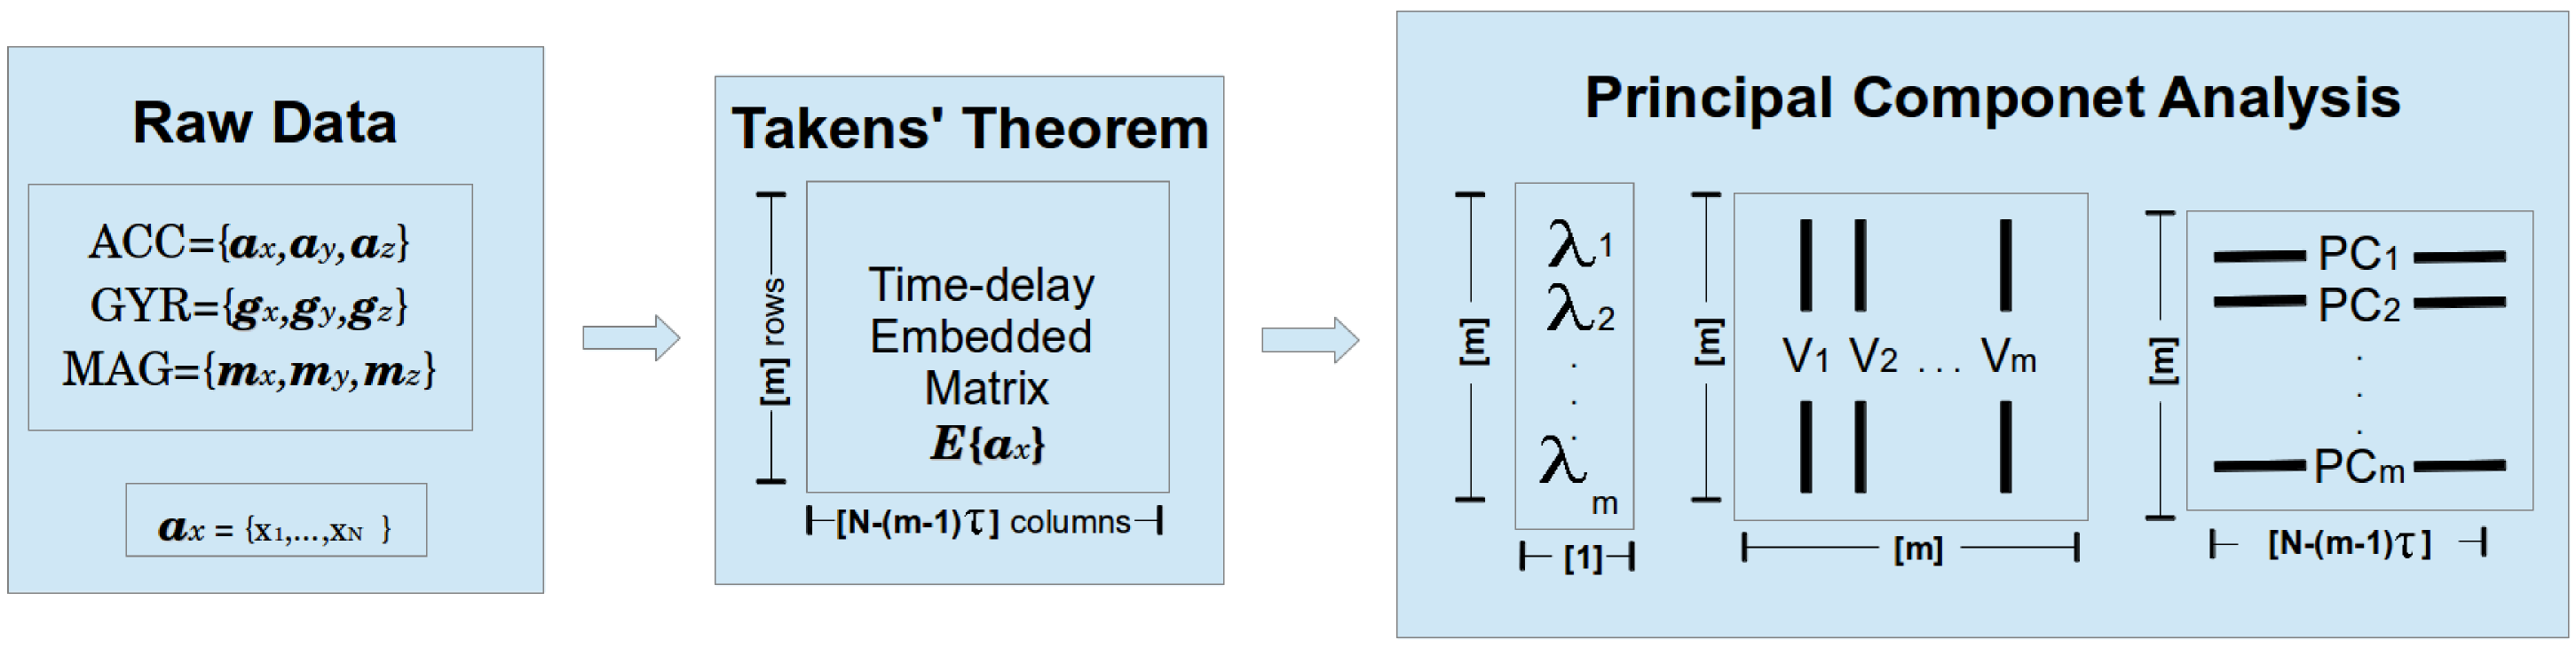
\includegraphics[width=\textwidth]{diagram_v9}
\caption[PA]{Diagram for the Phase Space Reconstruction.}
\label{fig:raw_takens_pca}
\end{figure*}


\subsection{Determining the minimum embedding dimension}
Although Takens's Theorem has been used extensevely in gait recognition and walking, running and cycling 
activities some problems are still remained to be solved.
For instance, Sama et al. \cite{Sama2013} estimated the minimal embedded dimension with False Nearest Neighbours (FNN) method.
However, Cao \cite{Cao1997} pointed out that FNN algorithm is subjective to different threshold parameters 
$R_{tol}$ and $A_{tol}$  which lead to different results and FNN method cannot differenciate random series 
from chaotic series. On the other hand, Frank et al. \cite{Frank2010} used a grid search 
to find the embedded parameters, but there are no details about their approach.
Additionally, Sama et al. \cite{Sama2013} states that the minimal embedding parameters largely depend on the 
application at hand, nevertheless there is still research to be done to find the minimal 
embedded parameters ($m$ and $\tau$).

\subsection{$E1(d)$ and $E2(d)$ values}
Cao's method for computing the minimal embedding dimmension is based on the mean values ($E1(d)$, $E2(d)$) of a
modified version of the FNN method, both values are only dependant on $m$ and $\tau$ \cite{Cao1997}.
$E1(d)$ is used to obtain the minimal dimmension and it stops changing when $d$ comes from an attractor.
On the other hand $E2(d)$ is used to distinguish deterministic signals from stochastic signals 
in which case the $E2(d)$ values will be approximately equal to 1 for any $d$.



\section{DATA COLLECTION}
Data from 3-axis accelerometer, gyroscope and magnetometer were collected at a sampling rate of 50 Hz 
using four Razor 9DOF IMUs with Bluetooth (Adeunis ARF7044). 
The IMUs were attached to custom-made bracelets worn by participants: 
two sensors were located in the front part of the right and left ankle, one in the 
back of the hip and another in back of the neck. 


\subsection{Participants}
Thirteen participants with different years of experience in dancing salsa were invited, one (male) 
expert dancer (14 years of experience), one intermediary (male) dancer (4 years of experience) 
and eleven non-dancers. 
The non-dancers were students of engineering (mean age 22 years; 4 female and 7 male).  
While 2 of these dancers (1 male and 1 female) had danced previously, none of this group had experience 
in Salsa dancing.  

\subsection{Experimental Conditions}
The design of the experiment met the University of XXX ethics approval and all participants provided informed 
consent prior to participation.

On arrival, participants were assisted in attaching the IMUs and the manner in which data were collected 
from these IMUs was demonstrated to them.  Once they were comforable with the fit of IMUs, 
the experimental task was explained to them.  

Each participant was shown a series of video clips (recorded by the expert dancer) demonstrating Salsa steps.  
Each video clip showed one step repeated several times for 20 seconds.  For the analysis in this paper, 
we report two Salsa step patterns (step 1 = mambo and step 2 = side crossover).  
Participants watched the video clip and were then asked to copy the steps in time to music.  
The video was played during the data collection 
(so that participants did not have to rely on their memory of the steps).

Data were collected from the IMUs and recorded.  
For this paper, the analysis reported will focus on data taken from the sensor mounted on the left ankle. 


\begin{table}
\tiny

  \centering
  
\begin{tabular}{l c c c c c c }
\toprule



& \multicolumn{6}{c}{Expert} \\
\cmidrule(r){2-7}

& \multicolumn{3}{c}{Step 1} & \multicolumn{3}{c}{Step 2}\\
\cmidrule(lr){2-4} \cmidrule(lr){5-7}

     & $C_1$  & $C_2$  & $C_1+C_2$  & $C_1$  & $C_2$  & $C_1+C_2$  \\
\midrule
% Percentega Of Variance

$\boldsymbol{E} a_{x}$ & 37.83 & 33.82 & 67.65 & 37.83 & 31.27 & 69.11 \\
$\boldsymbol{E} a_{y}$ & 18.12 & 17.20 & 35.32 & 30.49 & 23.99 & 54.48 \\
$\boldsymbol{E} a_{z}$ & 29.57 & 25.68 & 55.25 & 21.24 & 21.09 & 42.34 \\
$\boldsymbol{E} g_{x}$ & 29.98 & 24.89 & 54.87 & 32.73 & 27.68 & 60.42 \\
$\boldsymbol{E} g_{y}$ & 42.20 & 41.43 & 83.63 & 40.61 & 36.43 & 77.04 \\
$\boldsymbol{E} g_{z}$ & 40.07 & 36.18 & 76.25 & 43.32 & 41.38 & 84.71 \\
$\boldsymbol{E} m_{x}$ & 79.18 & 10.81 & 89.99 & 82.13 & 10.42 & 92.56 \\
$\boldsymbol{E} m_{y}$ & 67.43 & 9.03 & 76.46 & 73.31 & 21.00 & \cellcolor{blue!25}94.31 \\
$\boldsymbol{E} m_{z}$ & 66.36 & 28.19 & \cellcolor{blue!25}94.55 & 61.58 & 25.78 & 87.37   \\

\\
\\
& \multicolumn{6}{c}{Intermedium} \\
\cmidrule(r){2-7}

& \multicolumn{3}{c}{Step 1} & \multicolumn{3}{c}{Step 2}\\
\cmidrule(lr){2-4} \cmidrule(lr){5-7}
     & $C_1$  & $C_2$  & $C_1+C_2$  & $C_1$  & $C_2$  & $C_1+C_2$  \\
\midrule

$\boldsymbol{E} a_{x}$ & 37.51 & 32.28 & 69.79 & 23.11 & 22.17 & 45.28 \\
$\boldsymbol{E} a_{y}$ & 20.66 & 20.58 & 41.24 & 23.07 & 18.15 & 41.23 \\
$\boldsymbol{E} a_{z}$ & 32.77 & 29.85 & 62.62 & 14.35 & 13.65 & 28.00 \\
$\boldsymbol{E} g_{x}$ & 22.77 & 20.79 & 43.56 & 18.58 & 17.49 & 36.08 \\
$\boldsymbol{E} g_{y}$ & 46.85 & 40.58 & 87.43 & 40.32 & 39.21 & 79.53 \\
$\boldsymbol{E} g_{z}$ & 42.43 & 40.21 & 82.64 & 53.13 & 32.90 & 86.04 \\
$\boldsymbol{E} m_{x}$ & 84.91 & 9.40 & 94.31 & 81.80 & 15.01 & \cellcolor{blue!25}96.81 \\
$\boldsymbol{E} m_{y}$ & 64.00 & 28.66 & 92.66 & 77.41 & 18.17 & 95.59 \\
$\boldsymbol{E} m_{z}$ & 70.24 & 25.43 & \cellcolor{blue!25}95.67 & 79.29 & 16.45 & 95.75  \\

\\
\\
& \multicolumn{6}{c}{Non-dancer} \\
\cmidrule(r){2-7}

& \multicolumn{3}{c}{Step 1} & \multicolumn{3}{c}{Step 2}\\
\cmidrule(lr){2-4} \cmidrule(lr){5-7}
     & $C_1$  & $C_2$  & $C_1+C_2$  & $C_1$  & $C_2$  & $C_1+C_2$  \\
\midrule

$\boldsymbol{E} a_{x}$ & 26.41 & 21.57 & 47.98 & 31.27 & 23.92 & 55.20  \\
$\boldsymbol{E} a_{y}$ & 12.89 & 12.51 & 25.4 & 19.79 & 18.88 & 38.68 \\
$\boldsymbol{E} a_{z}$ & 15.12 & 14.84 & 29.96 & 20.22 & 18.75 & 38.98 \\
$\boldsymbol{E} g_{x}$ & 18.45 & 16.66 & 35.11 & 18.78 & 15.12 & 33.90 \\
$\boldsymbol{E} g_{y}$ & 44.11 & 38.84 & 82.95 & 43.20 & 33.99 & 77.20 \\
$\boldsymbol{E} g_{z}$ & 37.95 & 37.24 & 75.19 & 49.76 & 30.21 & 79.97 \\
$\boldsymbol{E} m_{x}$ & 64.24 & 23.82 & 88.06 & 83.79 & 12.43 & 96.23 \\
$\boldsymbol{E} m_{y}$ & 58.45 & 32.08 & 90.53 & 85.71 & 12.06 & \cellcolor{blue!25}97.77 \\
$\boldsymbol{E} m_{z}$ & 66.58 & 27.88 & \cellcolor{blue!25}94.46 & 72.99 & 20.96 & 93.96 \\

\bottomrule
\end{tabular}

  \caption{Percentages of variances of the first two PCA components and its addition
  %($C_1$, $C_2$, and $C_1 + C_2$)
  from the time-delay embedded matrices.
  Colored cells represent the maxium percentange of variation of the fist two components.}
  \label{tab:table1}
\end{table}




\section{DATA ANALYSIS}
Data from the inertial sensor for left ankle of the expert dancer were used to compute $E1(d)$ and $E2(d)$ values. 
$E1(d)$ and $E2(d)$ values are computed using a time-series ,for instance, $a_x$
so as to optain four curves that correspond to each delay embedding parameters ($\tau=1,2,3,4$)
for dimension that are in the range $0 \leq d \leq 40$.
From $E1(d)$ values 
(Figures~\ref{fig:e1acc},~\ref{fig:e1gyr} and ~\ref{fig:e1mag})
one can notice that the minimal value for the embedded dimmension is approximately
equal to $m=10$. 
  \begin{figure}[htbp!] 
  \centering    
  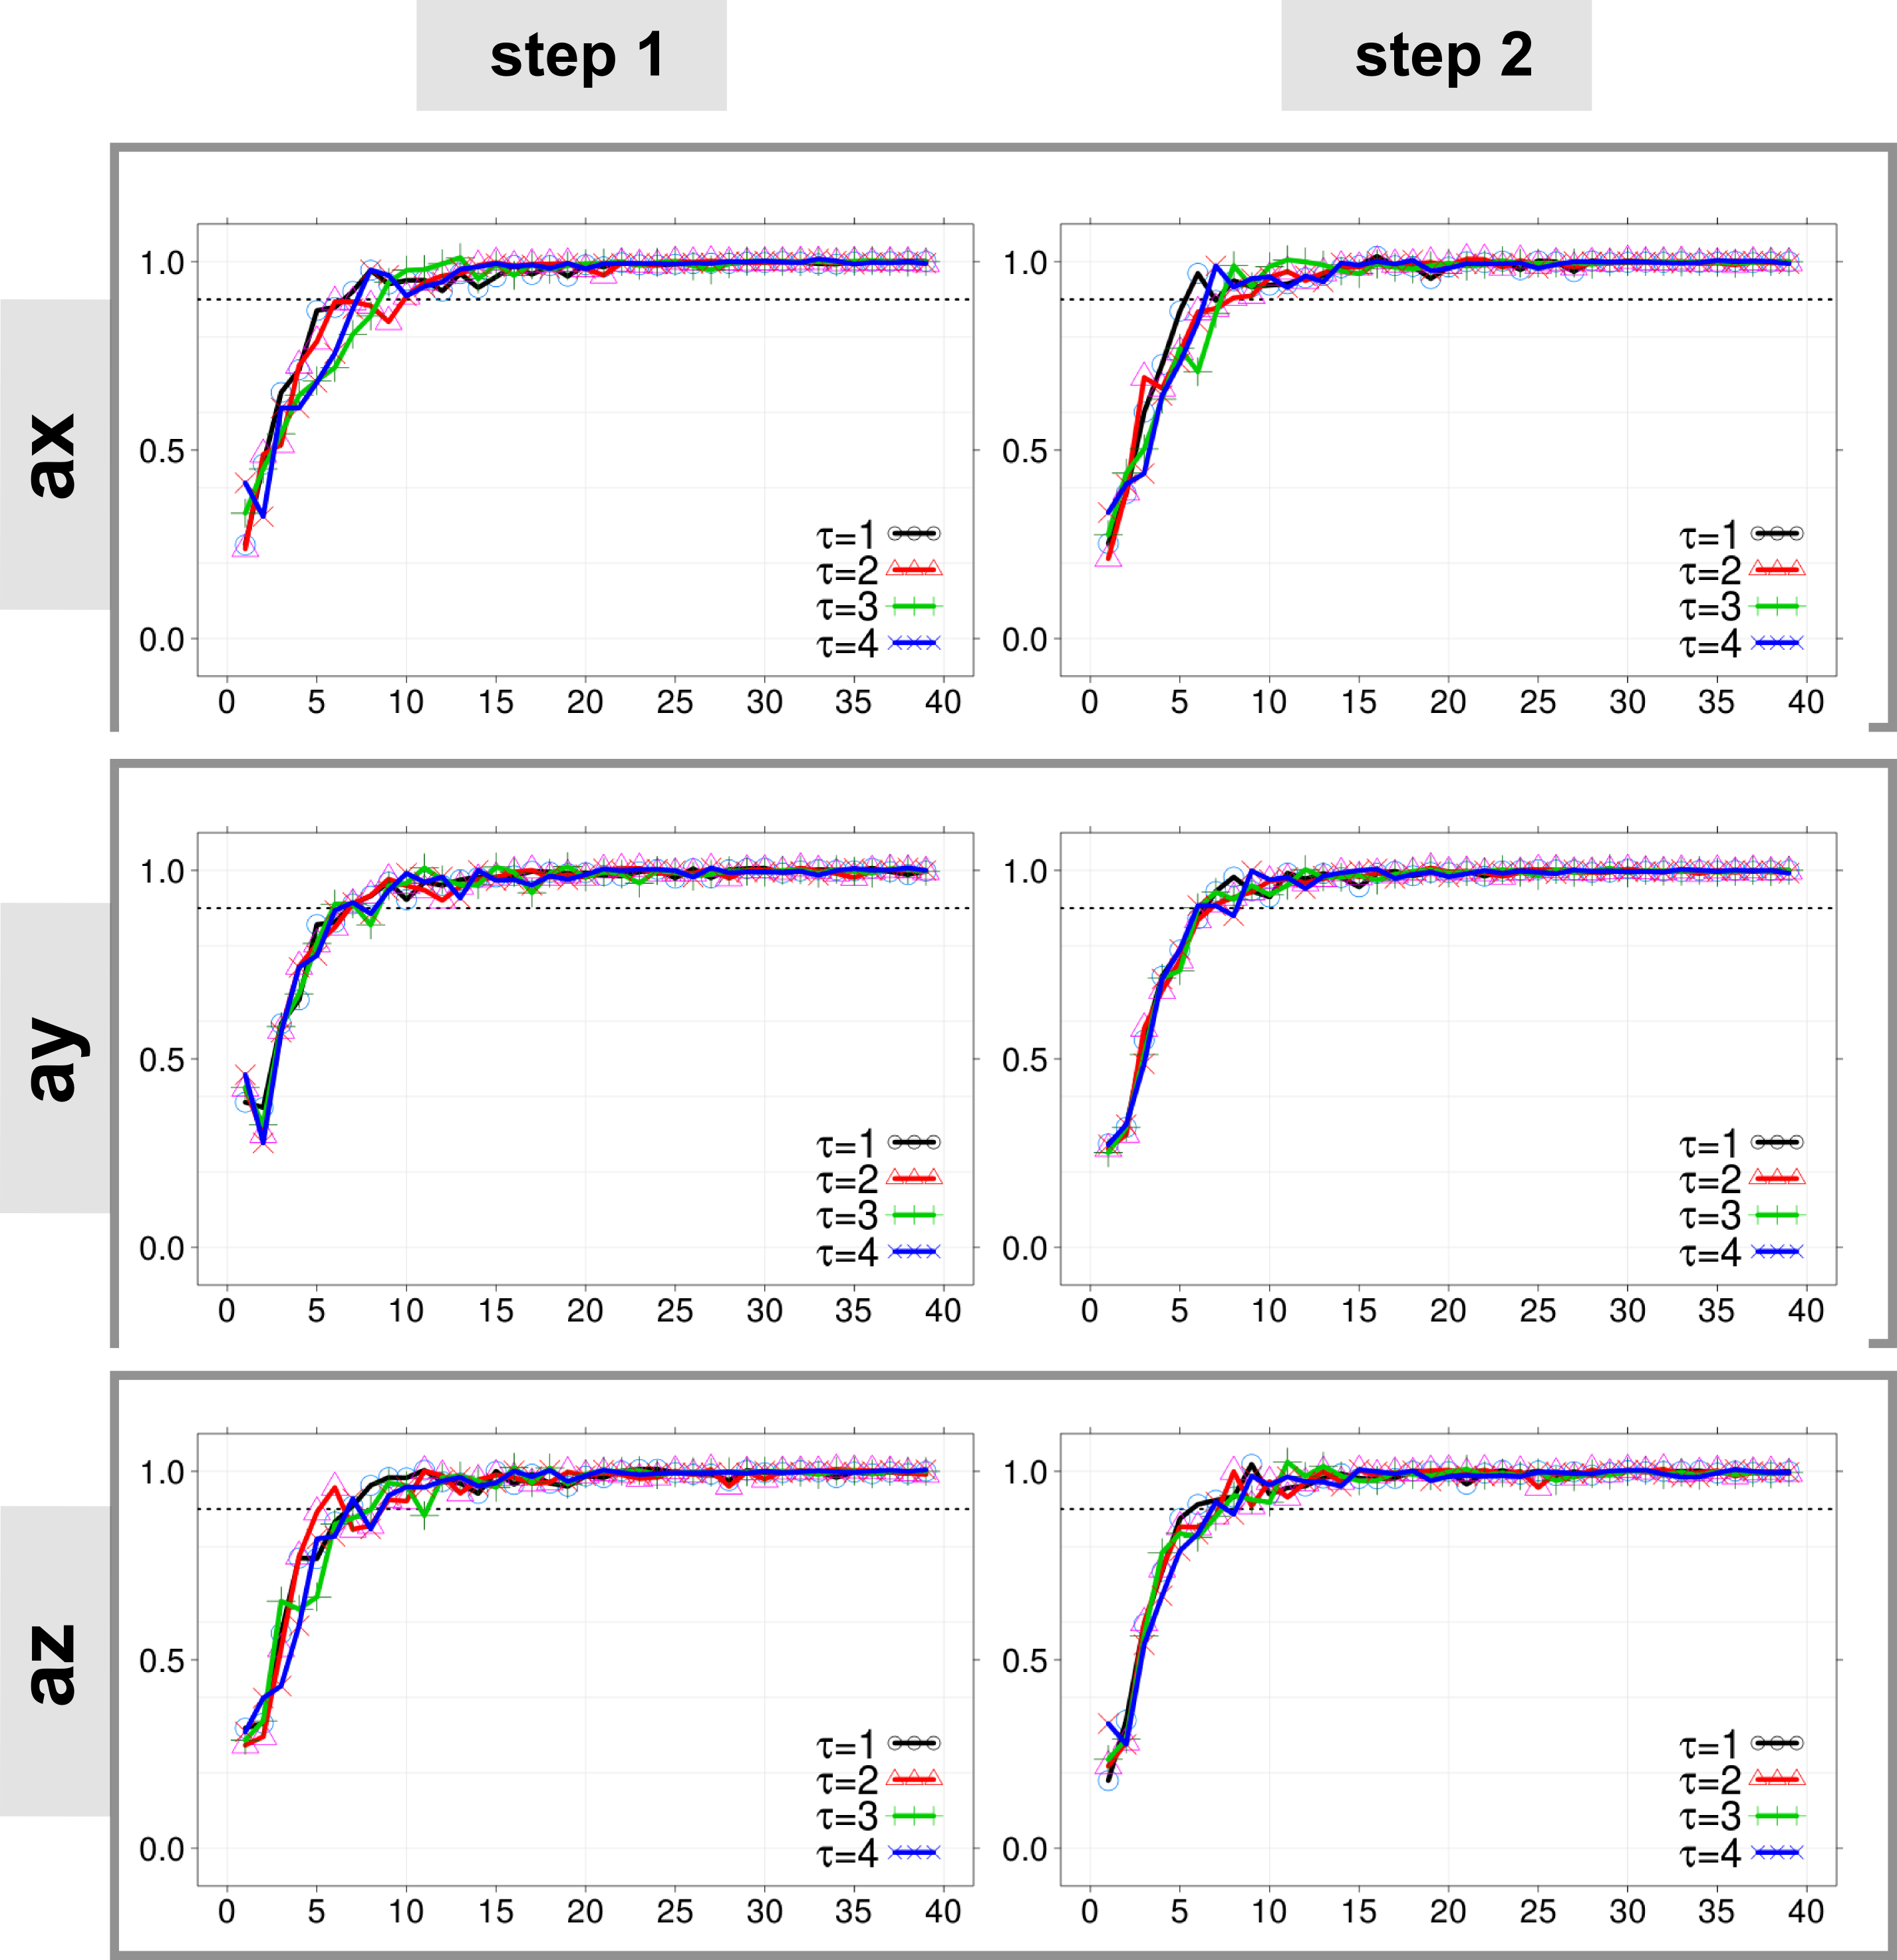
\includegraphics[width=0.45\textwidth]{e1_acc_expert}
  \caption[PA]{$E1(d)$ values for $\tau=1,2,3,4$ with $0 \leq d \leq 40$
  from the triaxial accelerometer of the expert dancer for two steps.}
  \label{fig:e1acc}
  \end{figure}
    \begin{figure}[htbp!] 
  \centering    
  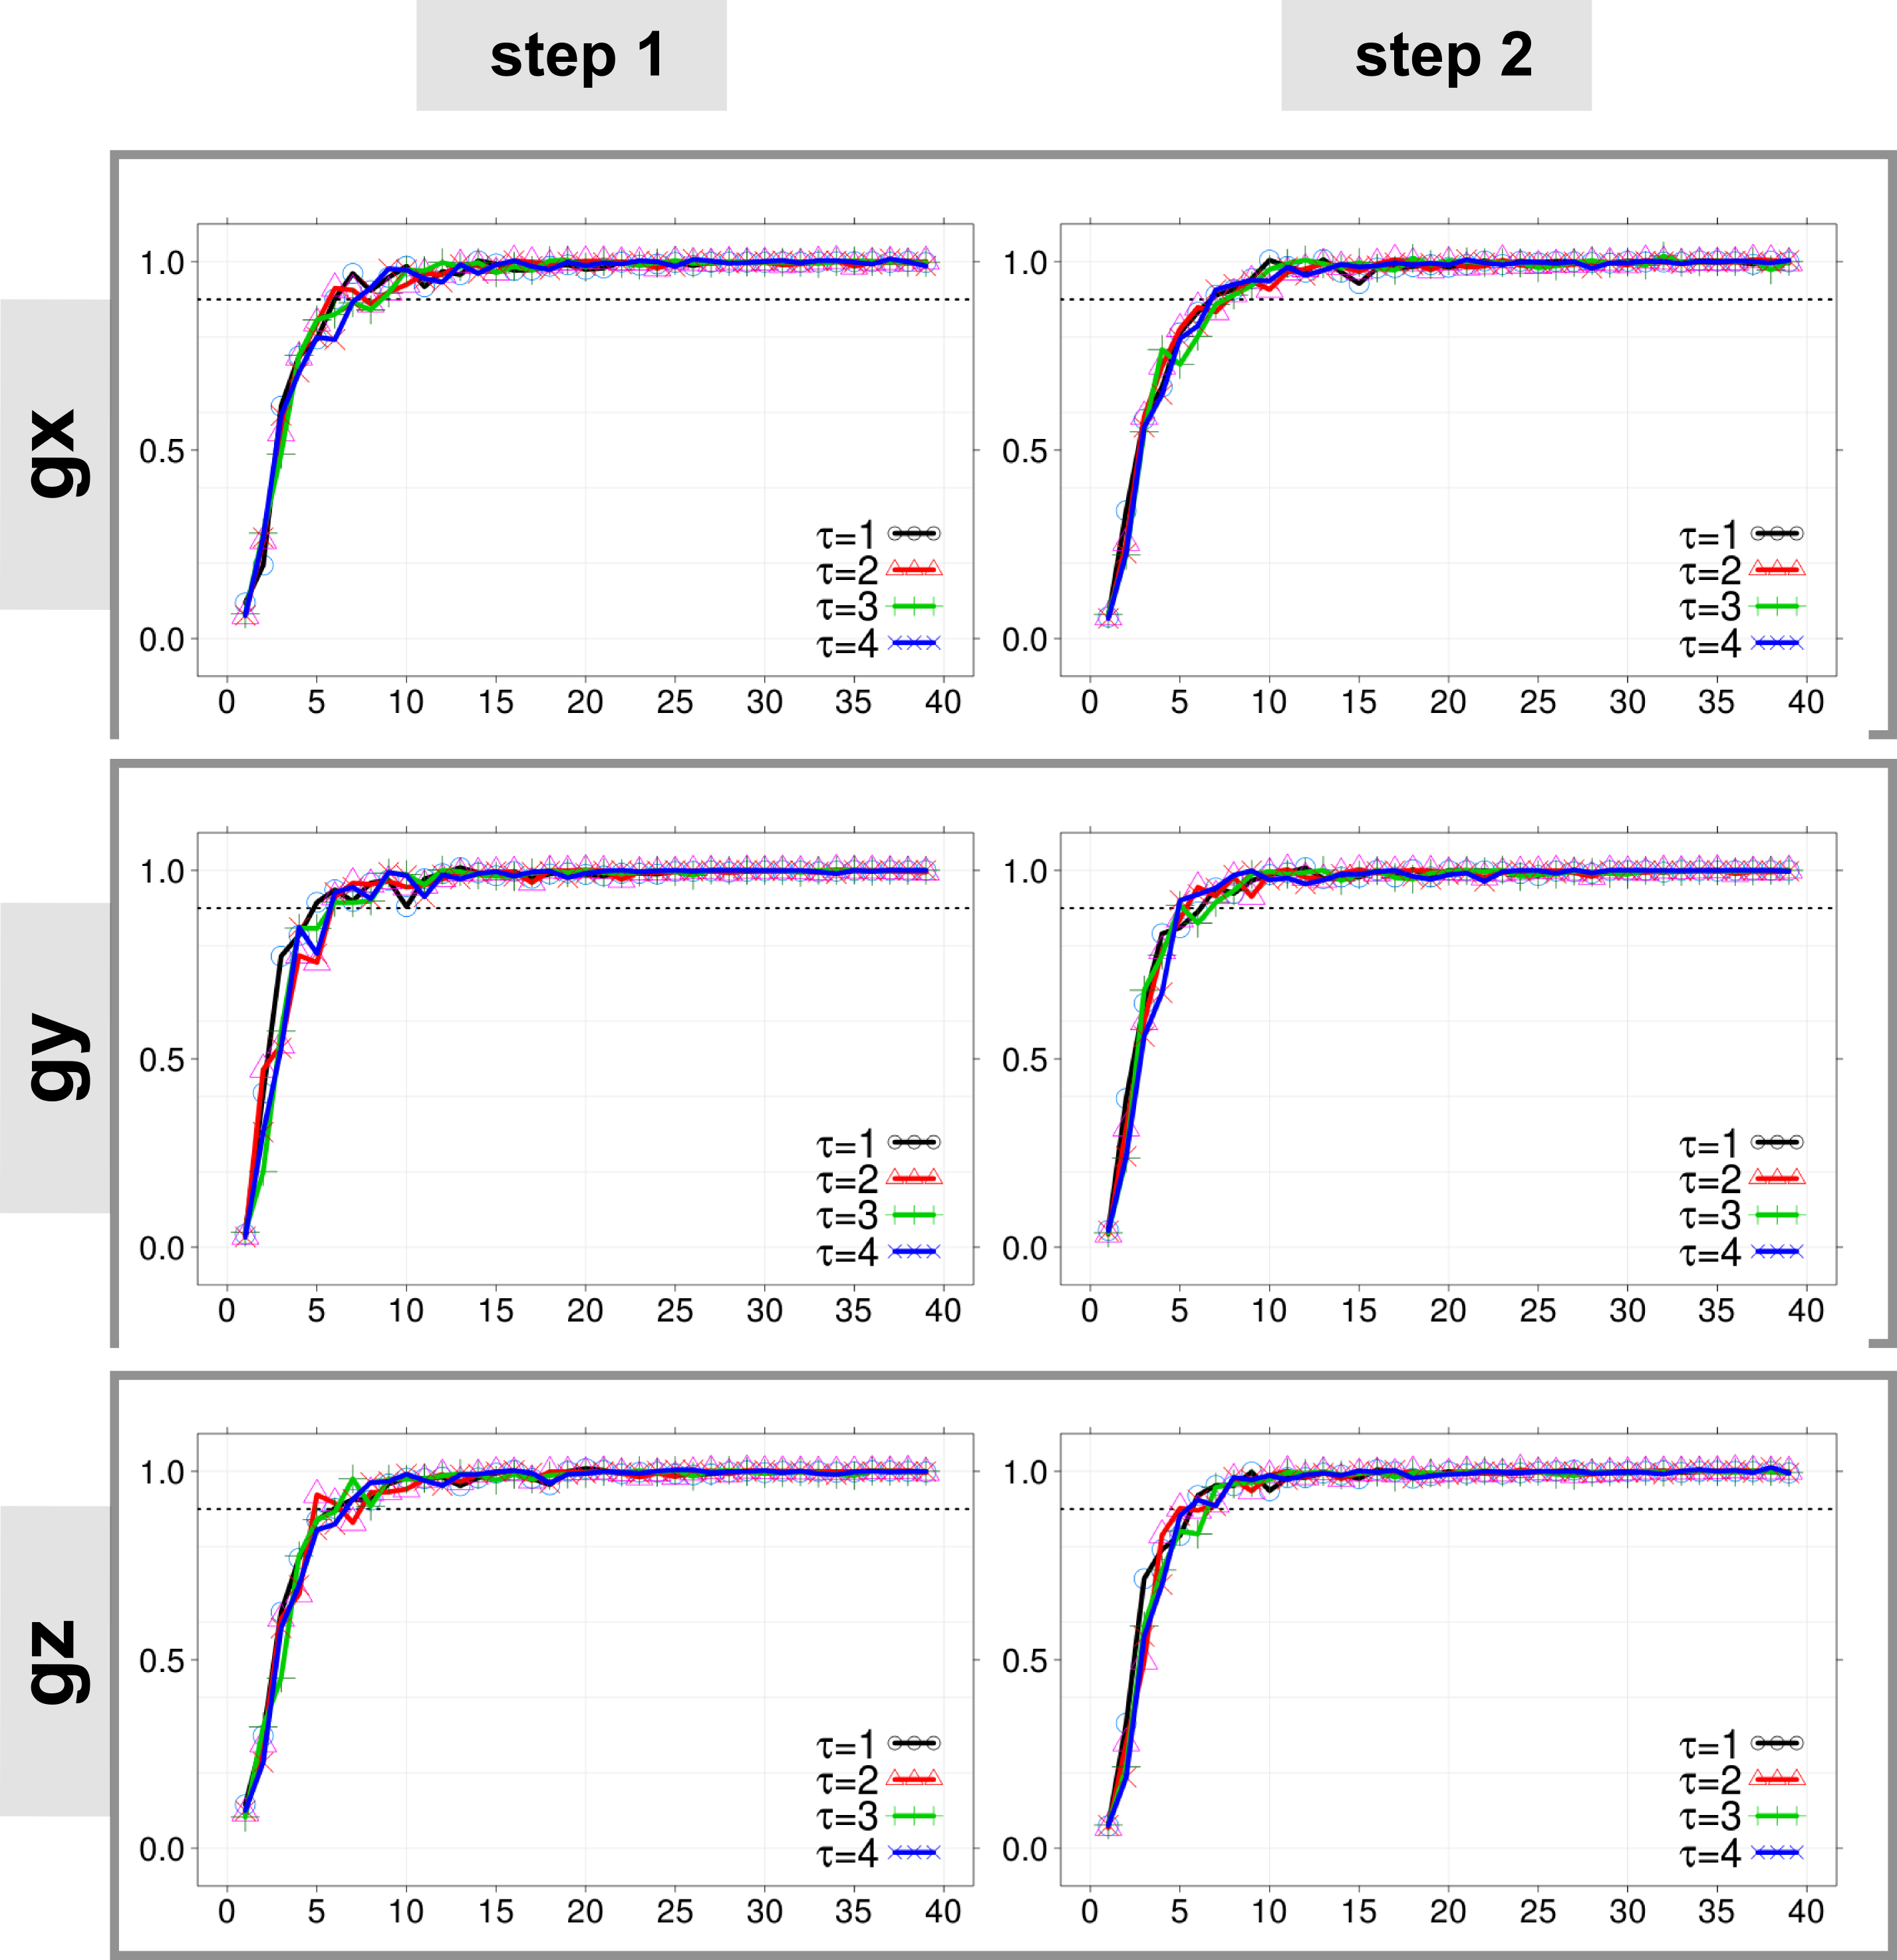
\includegraphics[width=0.45\textwidth]{e1_gyr_expert}
  \caption[PA]{$E1(d)$ values for $\tau=1,2,3,4$ with $0 \leq d \leq 40$
  from the triaxial gyroscope of the expert dancer for two steps.}
  \label{fig:e1gyr}
  \end{figure}
      \begin{figure}[htbp!] 
  \centering    
  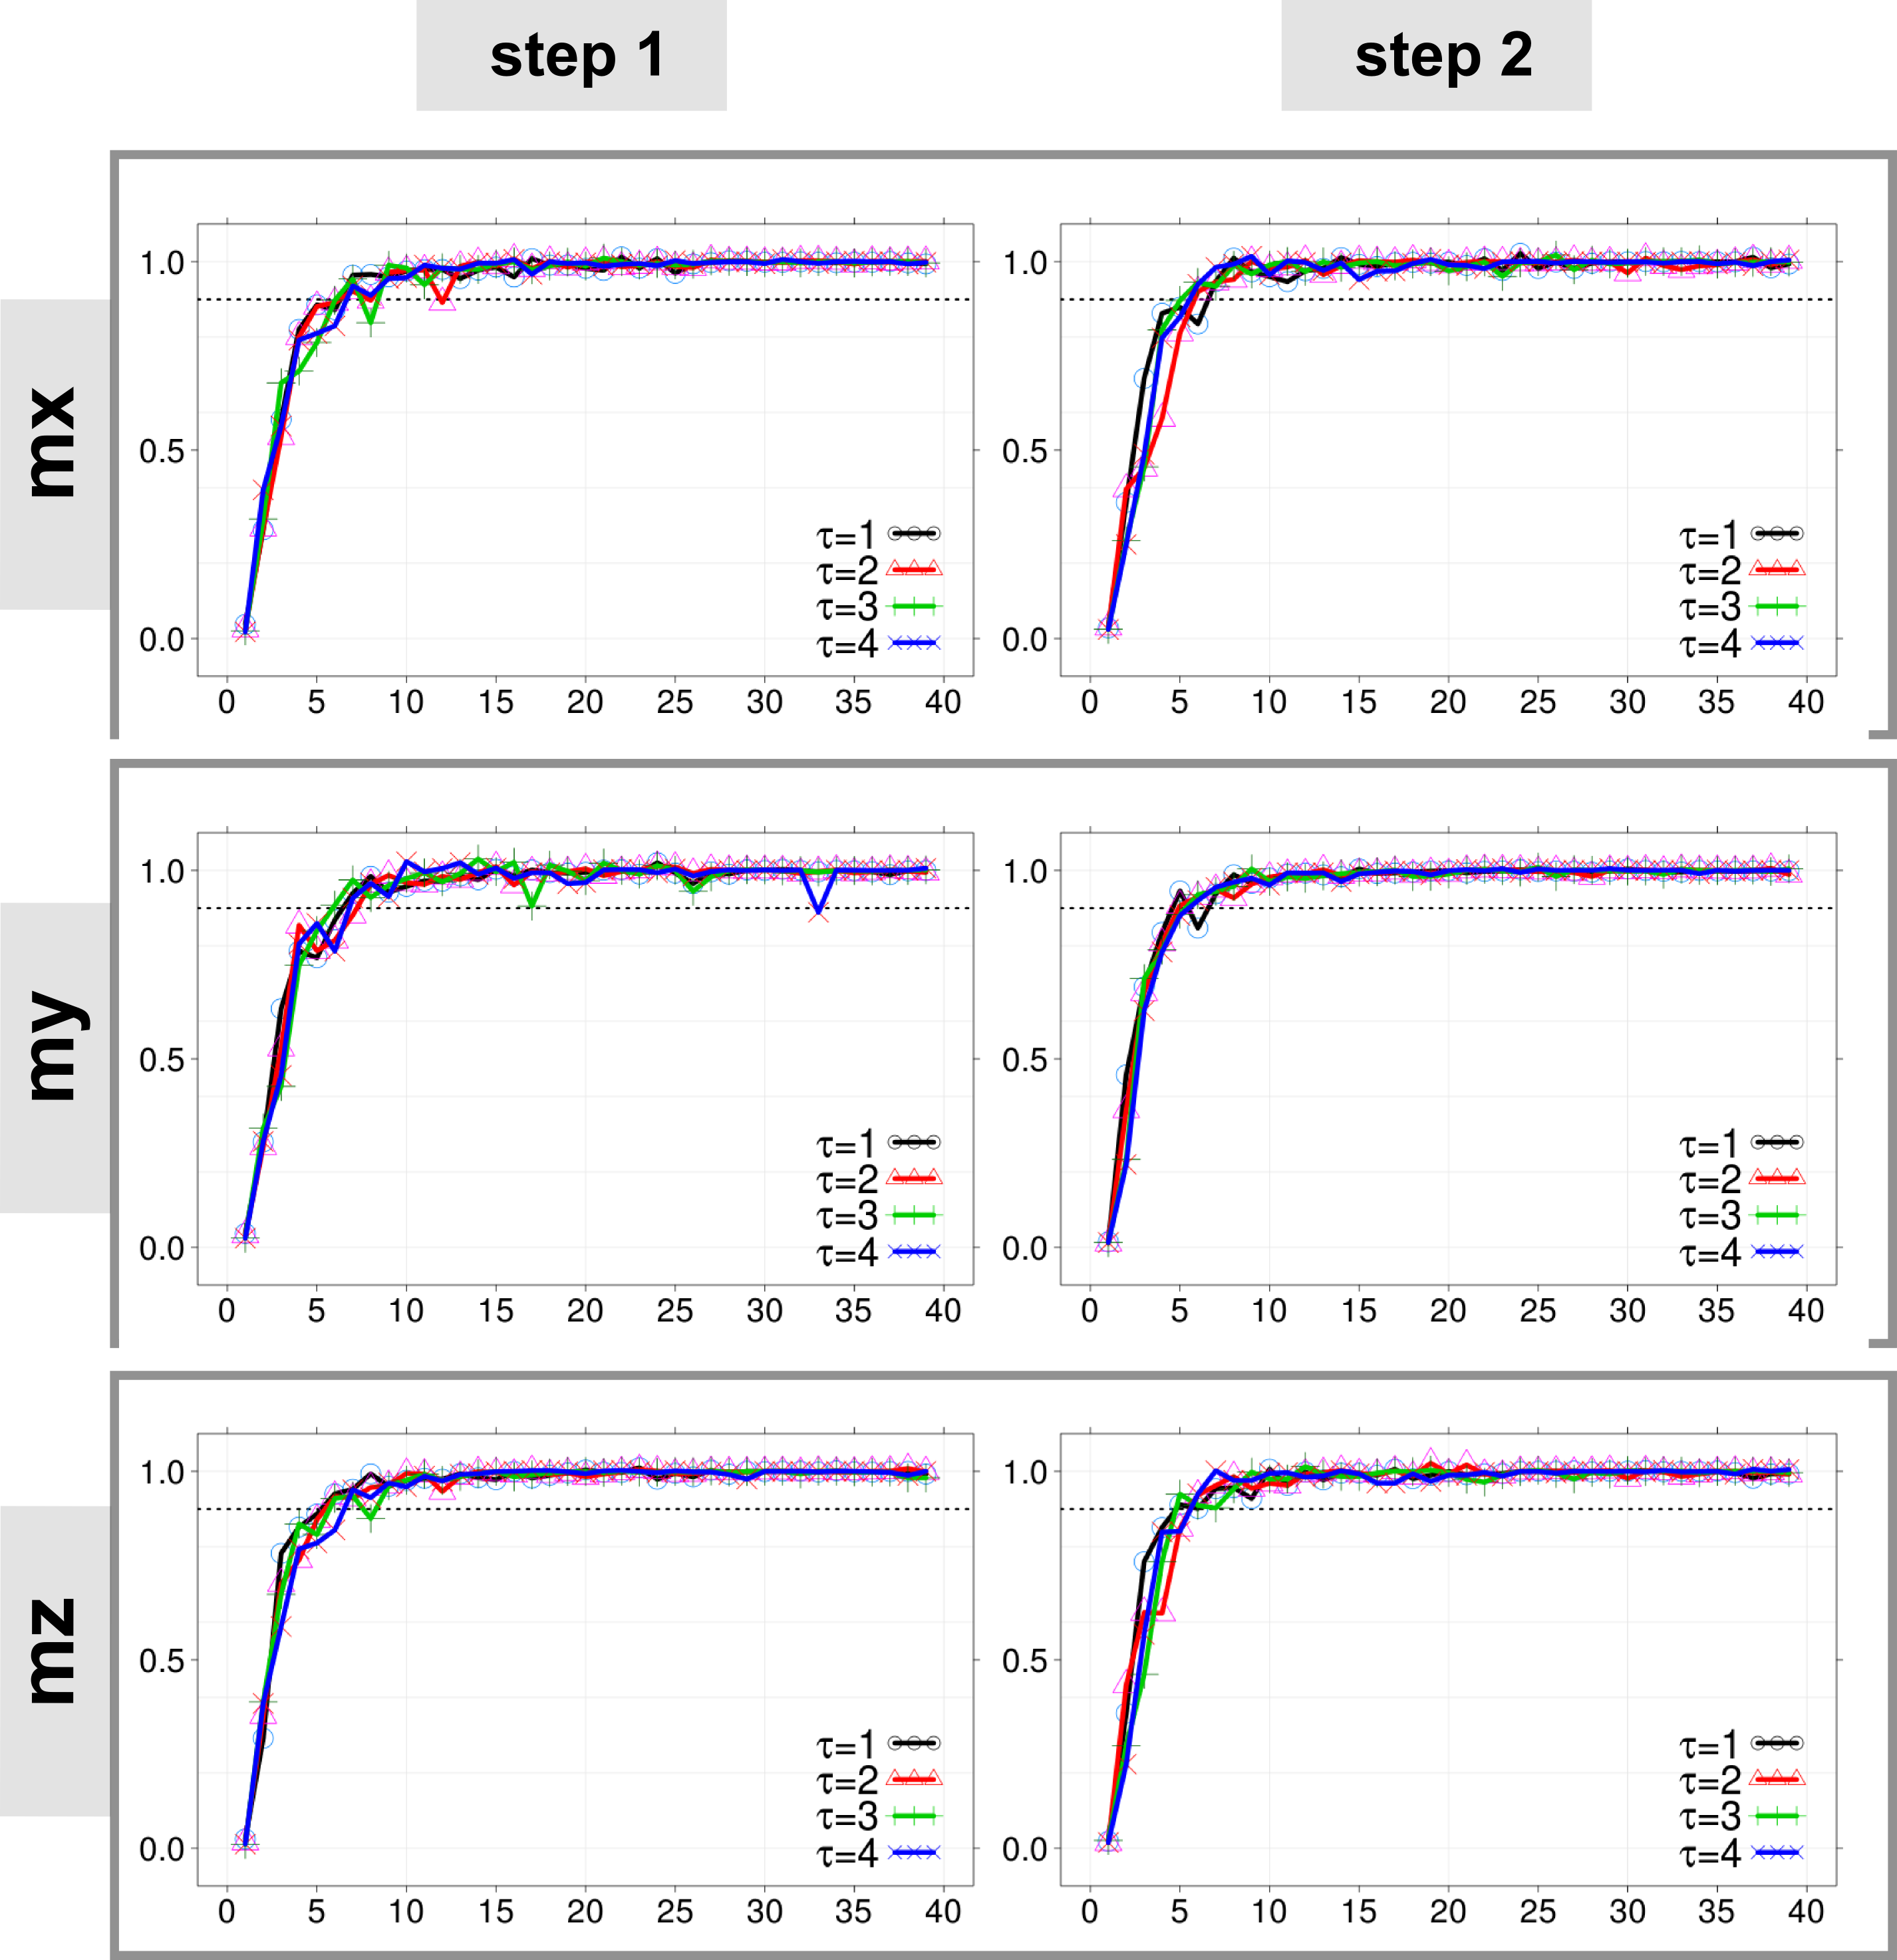
\includegraphics[width=0.45\textwidth]{e1_mag_expert}
  \caption[PA]{$E1(d)$ values for $\tau=1,2,3,4$ with $0 \leq d \leq 40$
  from the triaxial magnetometer of the expert dancer for two steps.}
  \label{fig:e1mag}
  \end{figure}
We define the minimal value as the point on the graph where the 
line appears to asymptote (or, at least, where the increase becomes very slight). 
It is important to note that neither the axis of the intertial sensor 
nor the time-delay values are a factor for having different embedded dimension parameters.
On the other hand, from $E2(d)$ values (Figures~\ref{fig:e2acc},~\ref{fig:e2gyr} and ~\ref{fig:e2mag})
one can appreciate that the accelerometer data is more random since their values are closer to 1
which is also the case for the x-axis in the gyroscope and magnetometer sensor. 
Fortunately, y and z axis in the gyroscope and magnetometer provide more deterministic data.
    \begin{figure}[htbp!] 
  \centering    
  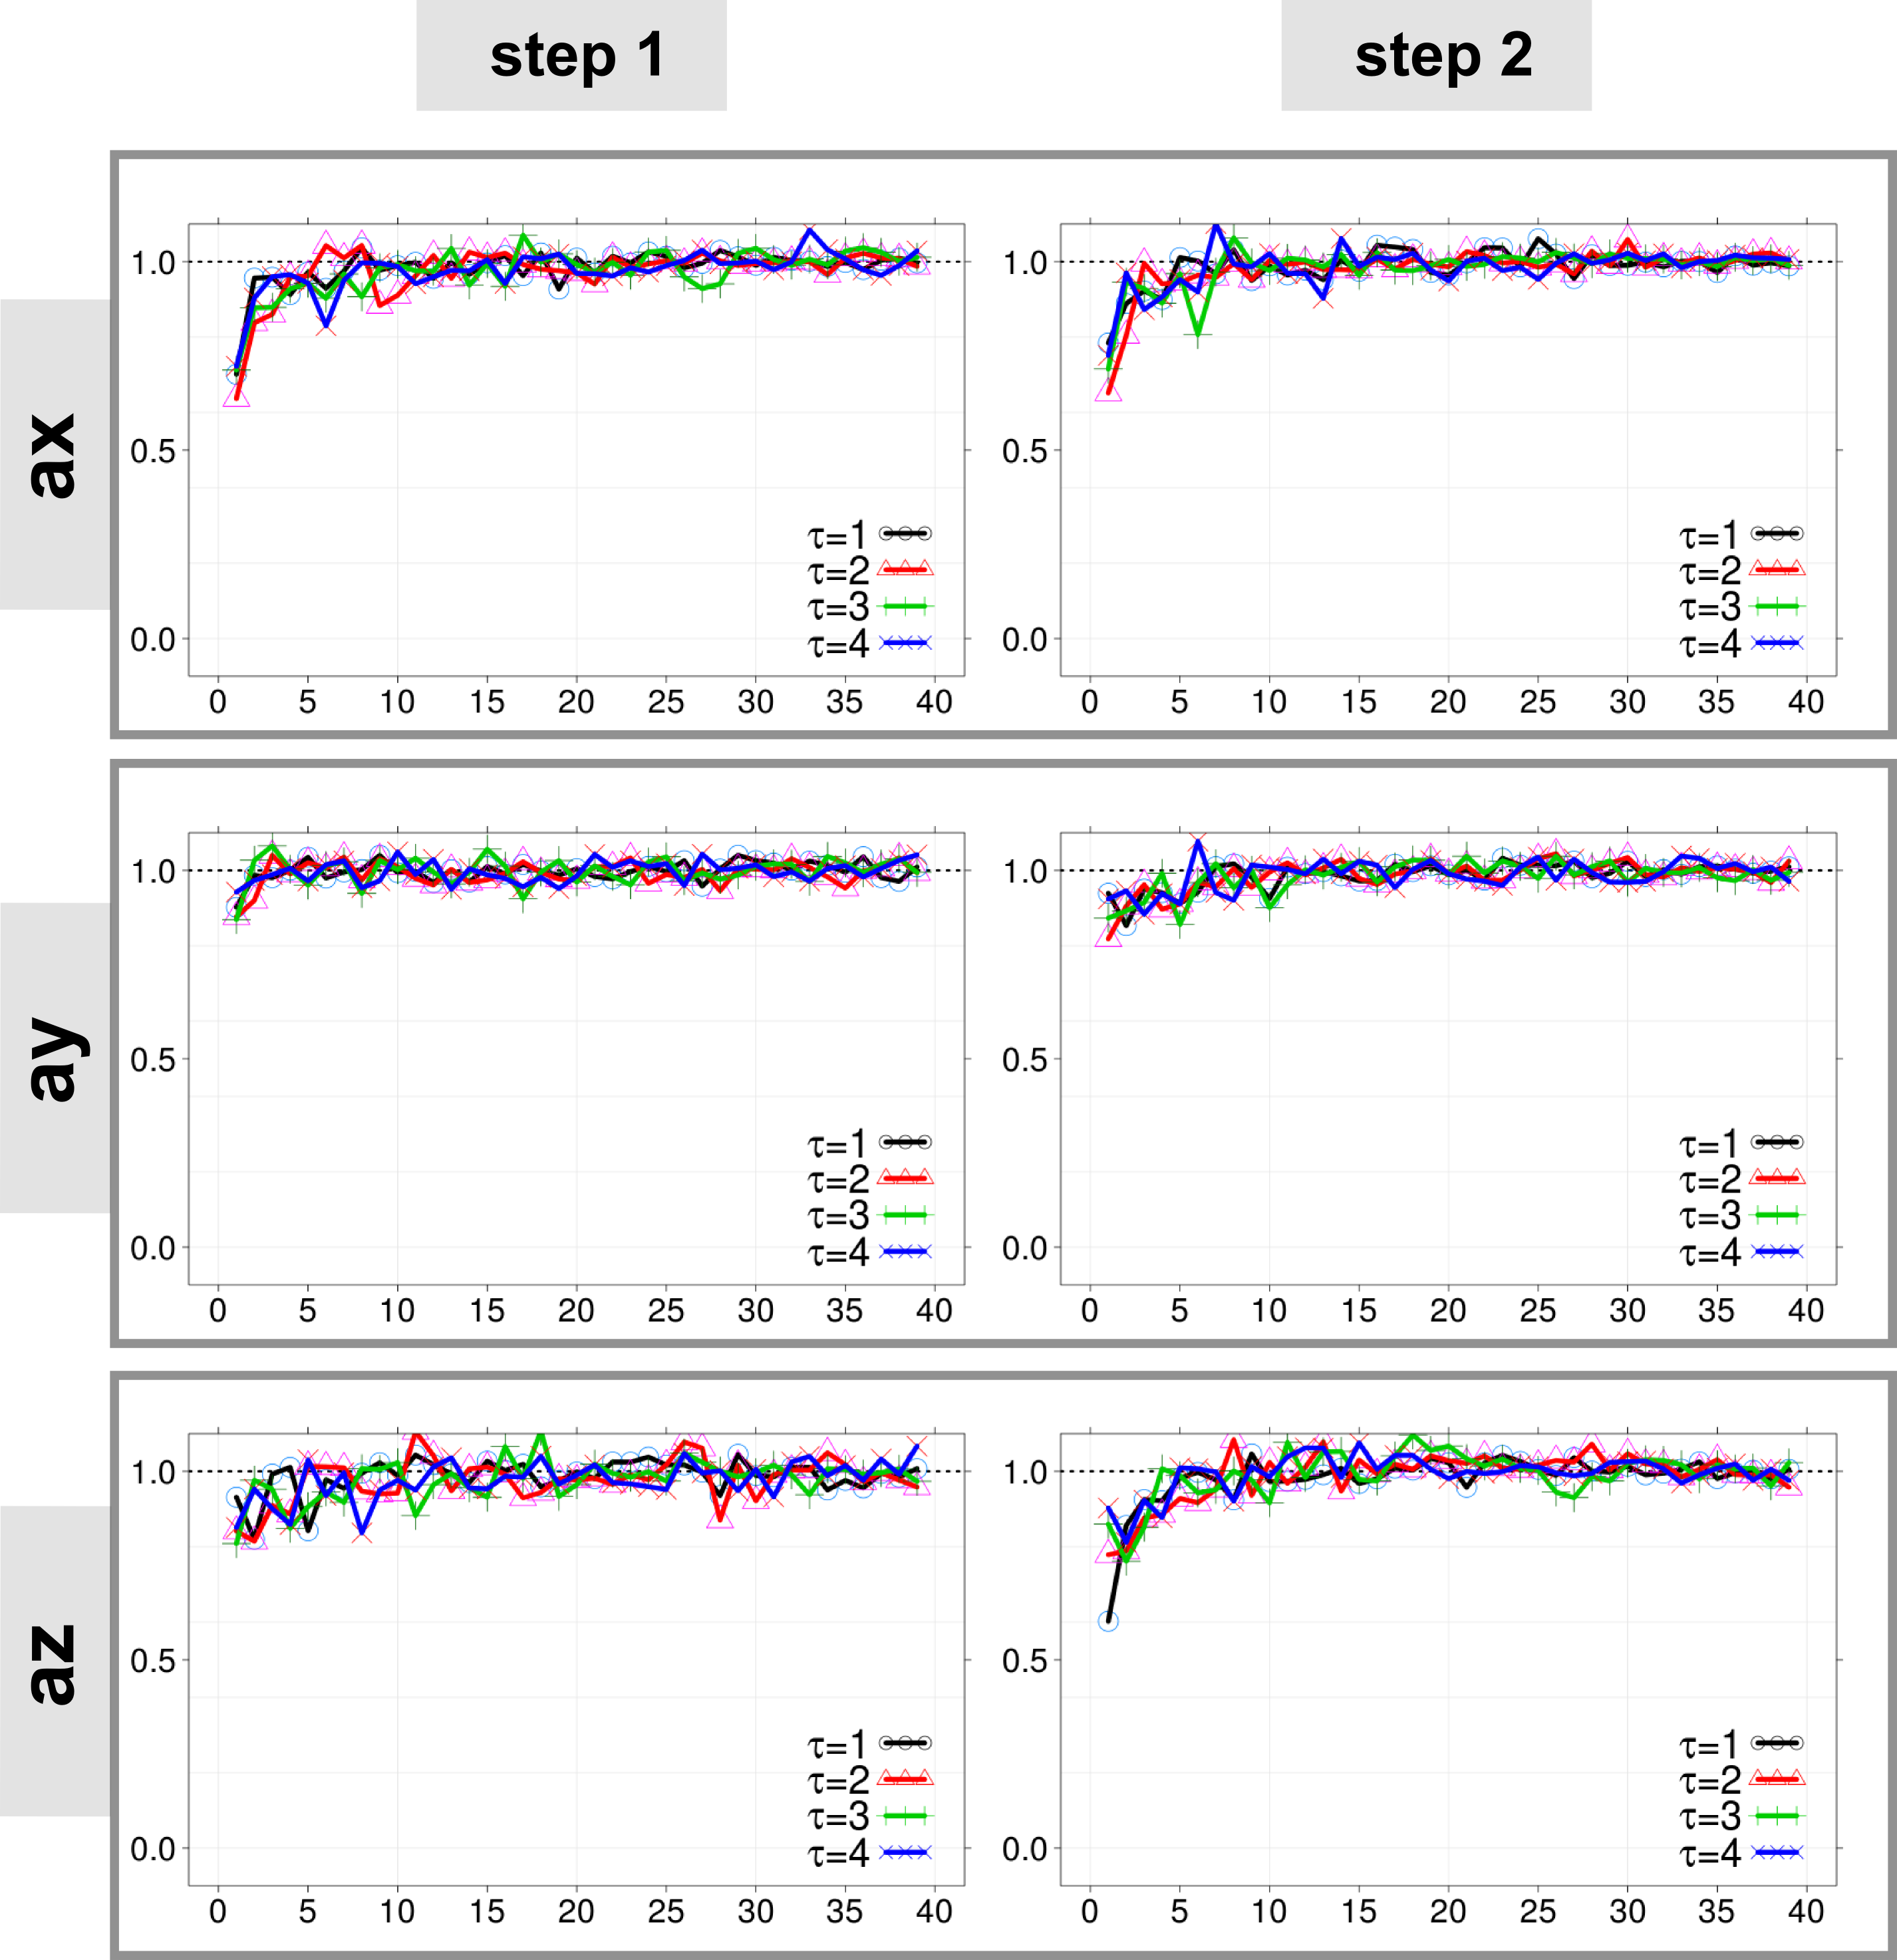
\includegraphics[width=0.45\textwidth]{e2_acc_expert}
  \caption[PA]{$E2(d)$ values for $\tau=1,2,3,4$ with $0 \leq d \leq40 $
  from the triaxial accelerometer of the expert dancer for two steps.
  %If $E2(d)$ values are approximately equal to 1 for any $d$ the time serie is random.
  }
  \label{fig:e2acc}
  \end{figure}
      \begin{figure}[htbp!] 
  \centering    
  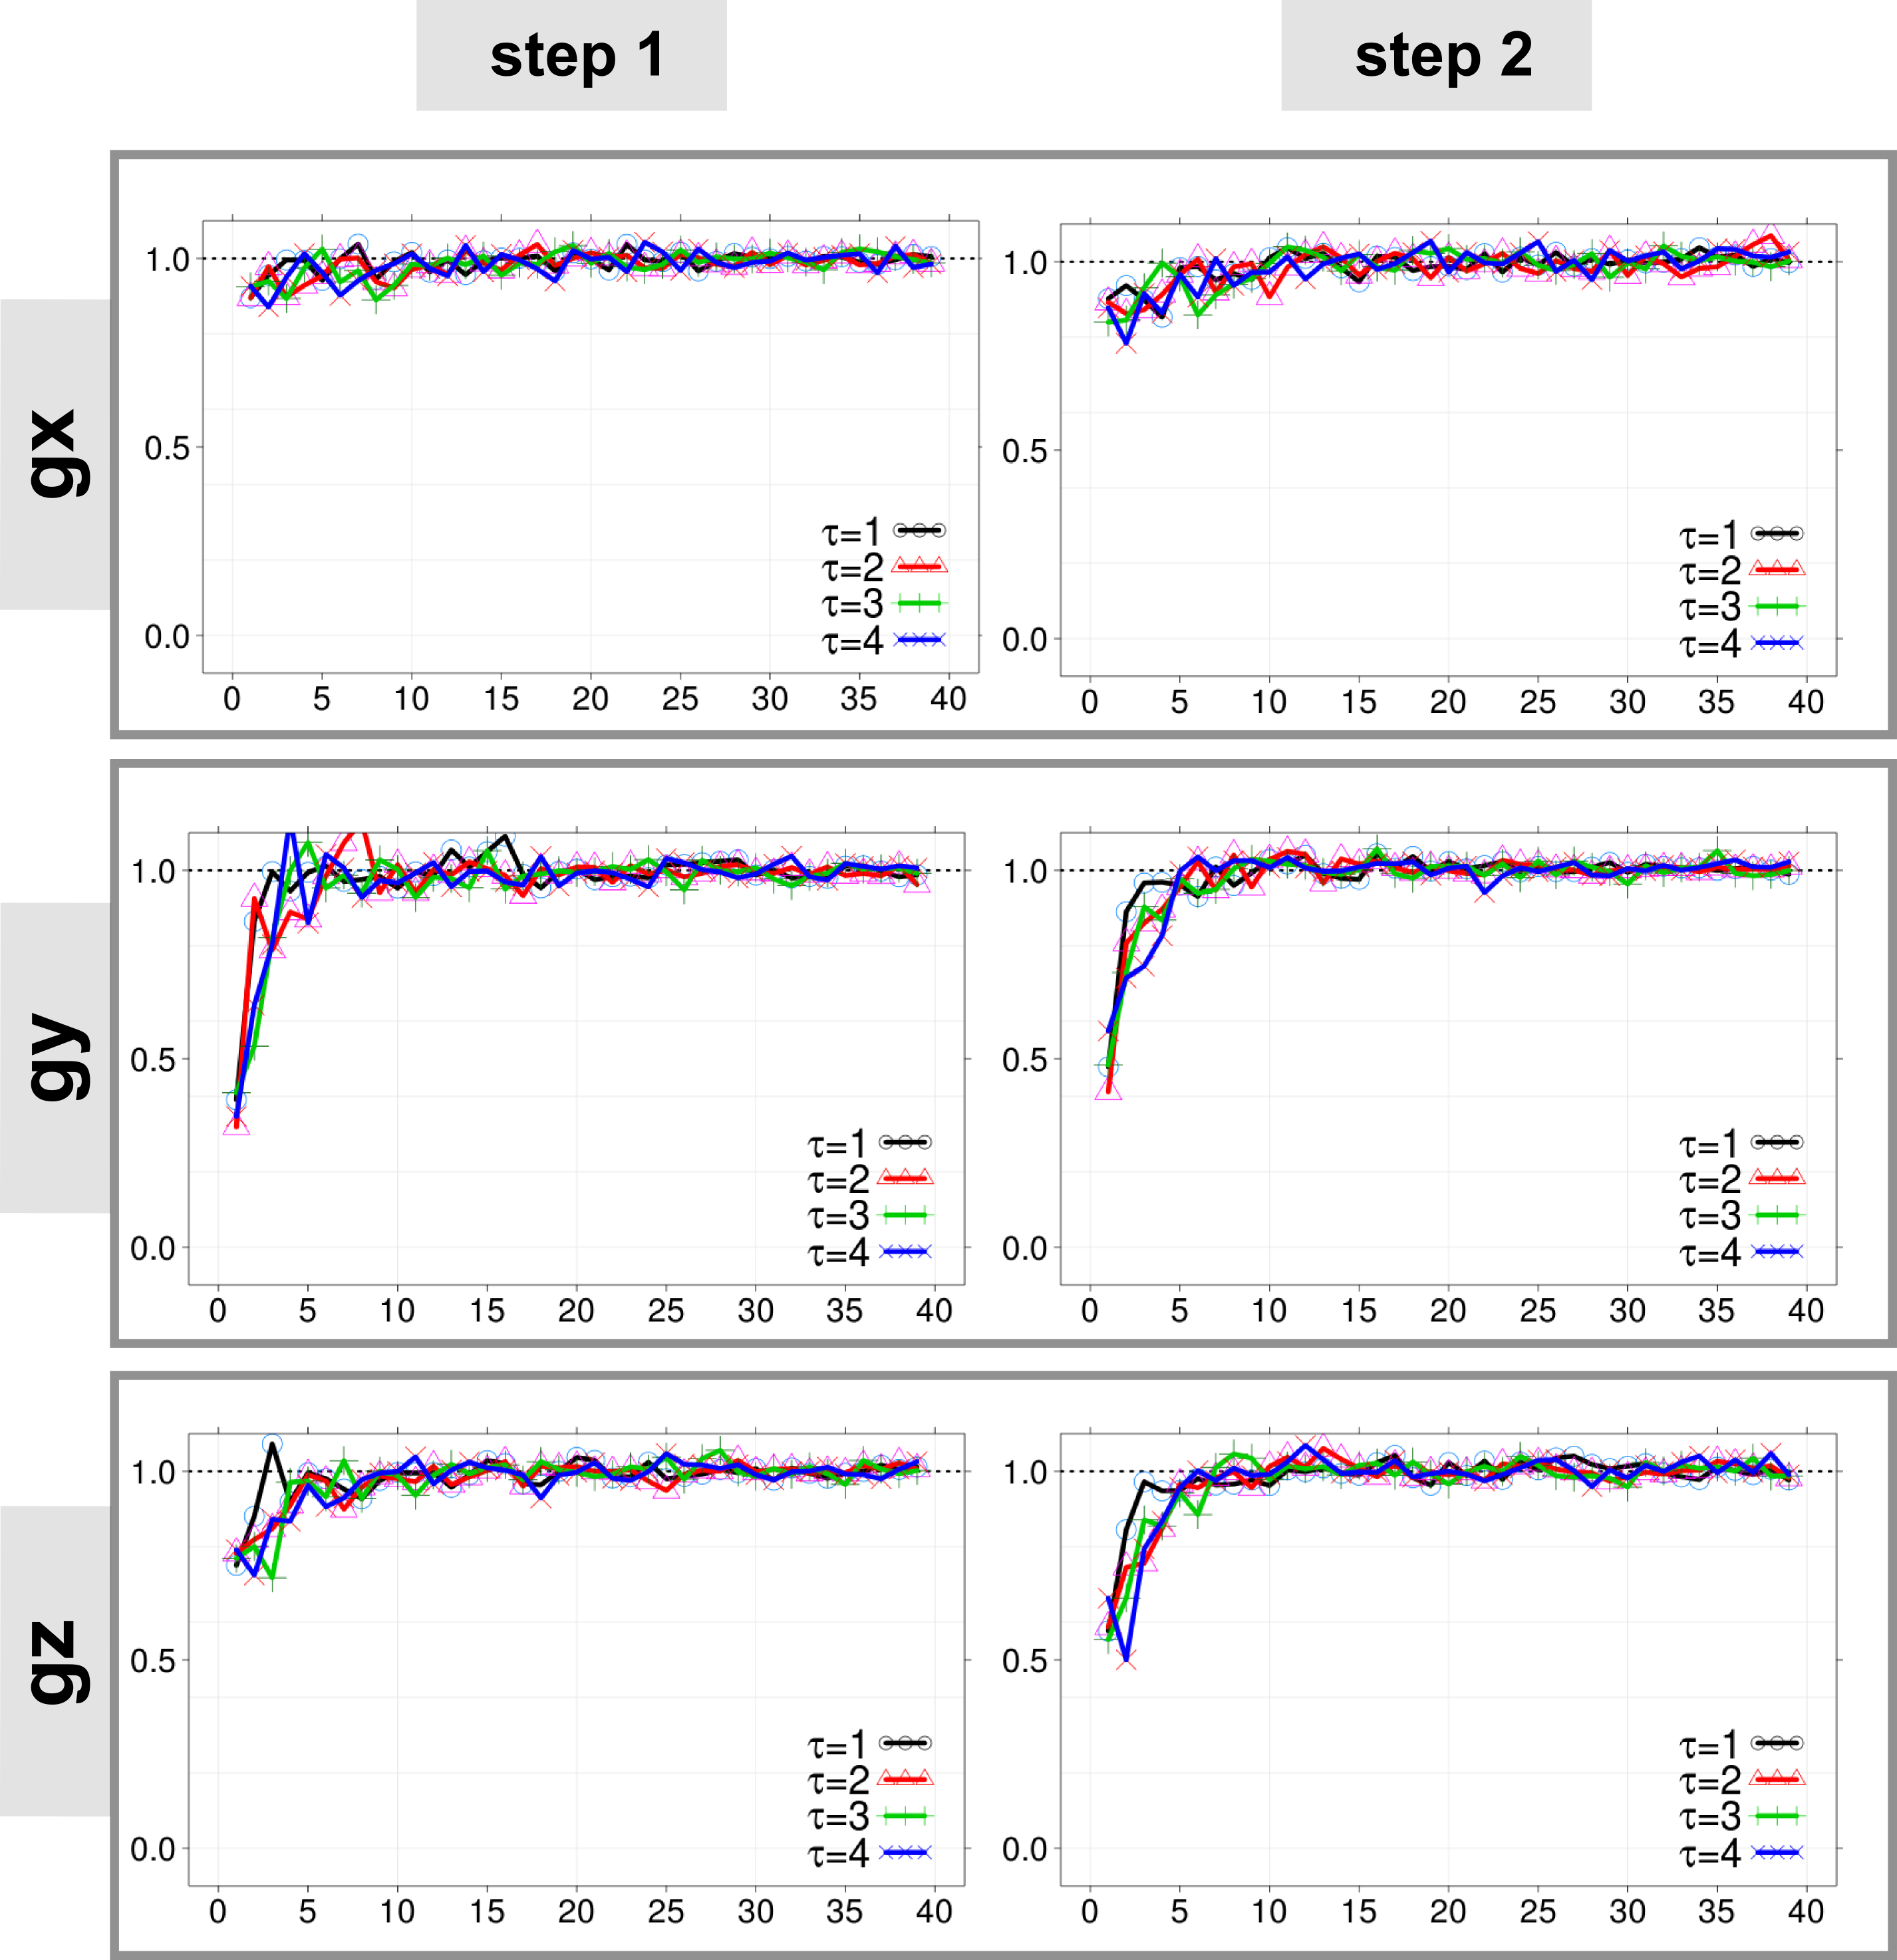
\includegraphics[width=0.45\textwidth]{e2_gyr_expert}
  \caption[PA]{$E2(d)$ values for $\tau=1,2,3,4$ with $0 \leq d \leq40 $
  from the triaxial gyroscope of the expert dancer for two steps.
  %If $E2(d)$ values are approximately equal to 1 for any $d$ the time serie is random.
  }
  \label{fig:e2gyr}
  \end{figure}
      \begin{figure}[htbp!] 
  \centering    
  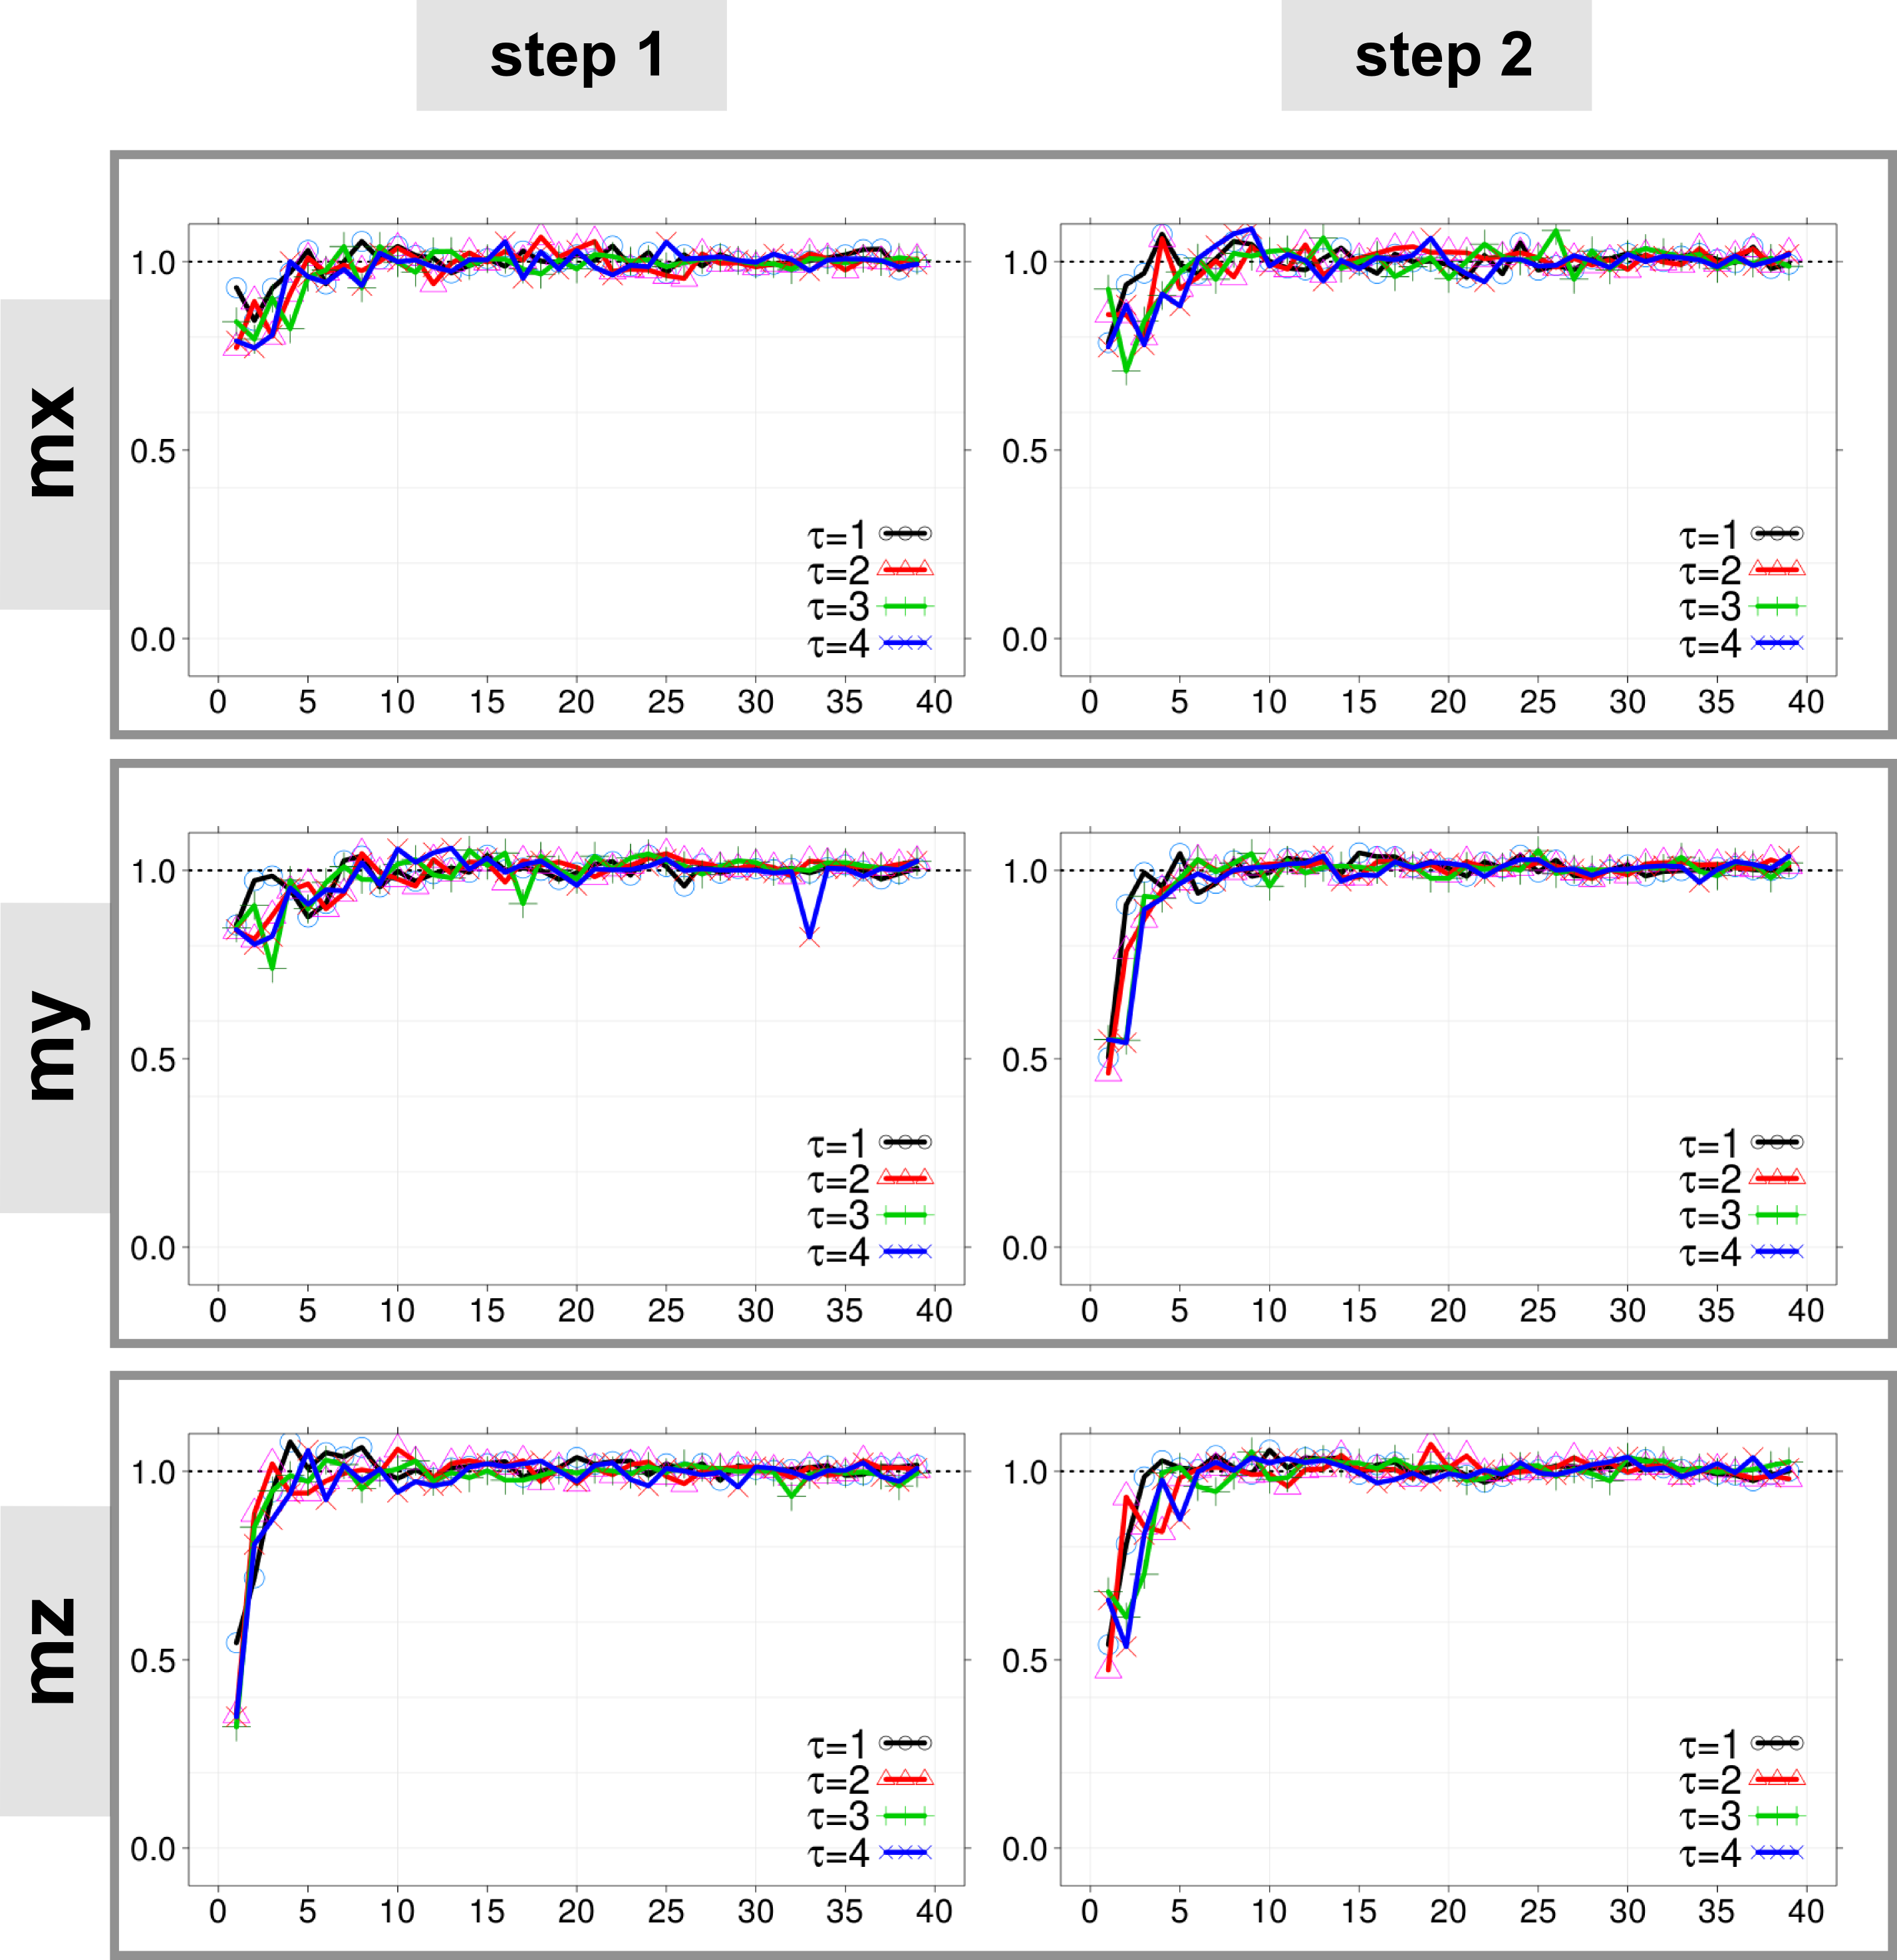
\includegraphics[width=0.45\textwidth]{e2_mag_expert}
  \caption[PA]{$E2(d)$ values for $\tau=1,2,3,4$ with $0 \leq d \leq40 $
  from the triaxial magnetometer of the expert dancer for two steps.
  %If $E2(d)$ values are approximately equal to 1 for any $d$ the time serie is random.
  }
  \label{fig:e2mag}
  \end{figure}  

Independenly of the sensors' axis or dance steps, different $\tau$ values provide approximately the 
same minimal embeding dimension ($m=10$) in $E1(d)$ values (Figures~\ref{fig:e1acc},~\ref{fig:e1gyr} and ~\ref{fig:e1mag}).
We therefore computed the Takens' Theorem 
with $m=10$ and $\tau = 1$ for each axis of the IMU as depicted in Figure \ref{fig:raw_takens_pca}.
Table~\ref{tab:table1} illustrates the first two components and its addition values of the PCA ($C_1$, $C_2$, $C_1+ C_2$)
using all embedded matrix axis ($Ea_{ \{ x,y,z \} },Eg_{\{ x,y,z \}},Em_{\{ x,y,z \}}$) for step 1 and step 2 from expert, 
intermedium and non-dancer participants.
Table~\ref{tab:table1} also help us to select the sensor and the axis that 
provides the highest variance in the data.
We therefore choose the magnetometer sensor in the z-axis since it has the highest variance for step 1
and the magnetometer sensor in the y-axis in the case of the step 2.

Additionally, we illustrate the problem of the minimal embedded parameters since 
different pairs of embedded parameters might be used to reconstruct the state space (Figure ~\ref{fig:takens_problem}). 
\begin{figure}[htbp!] 
\centering    
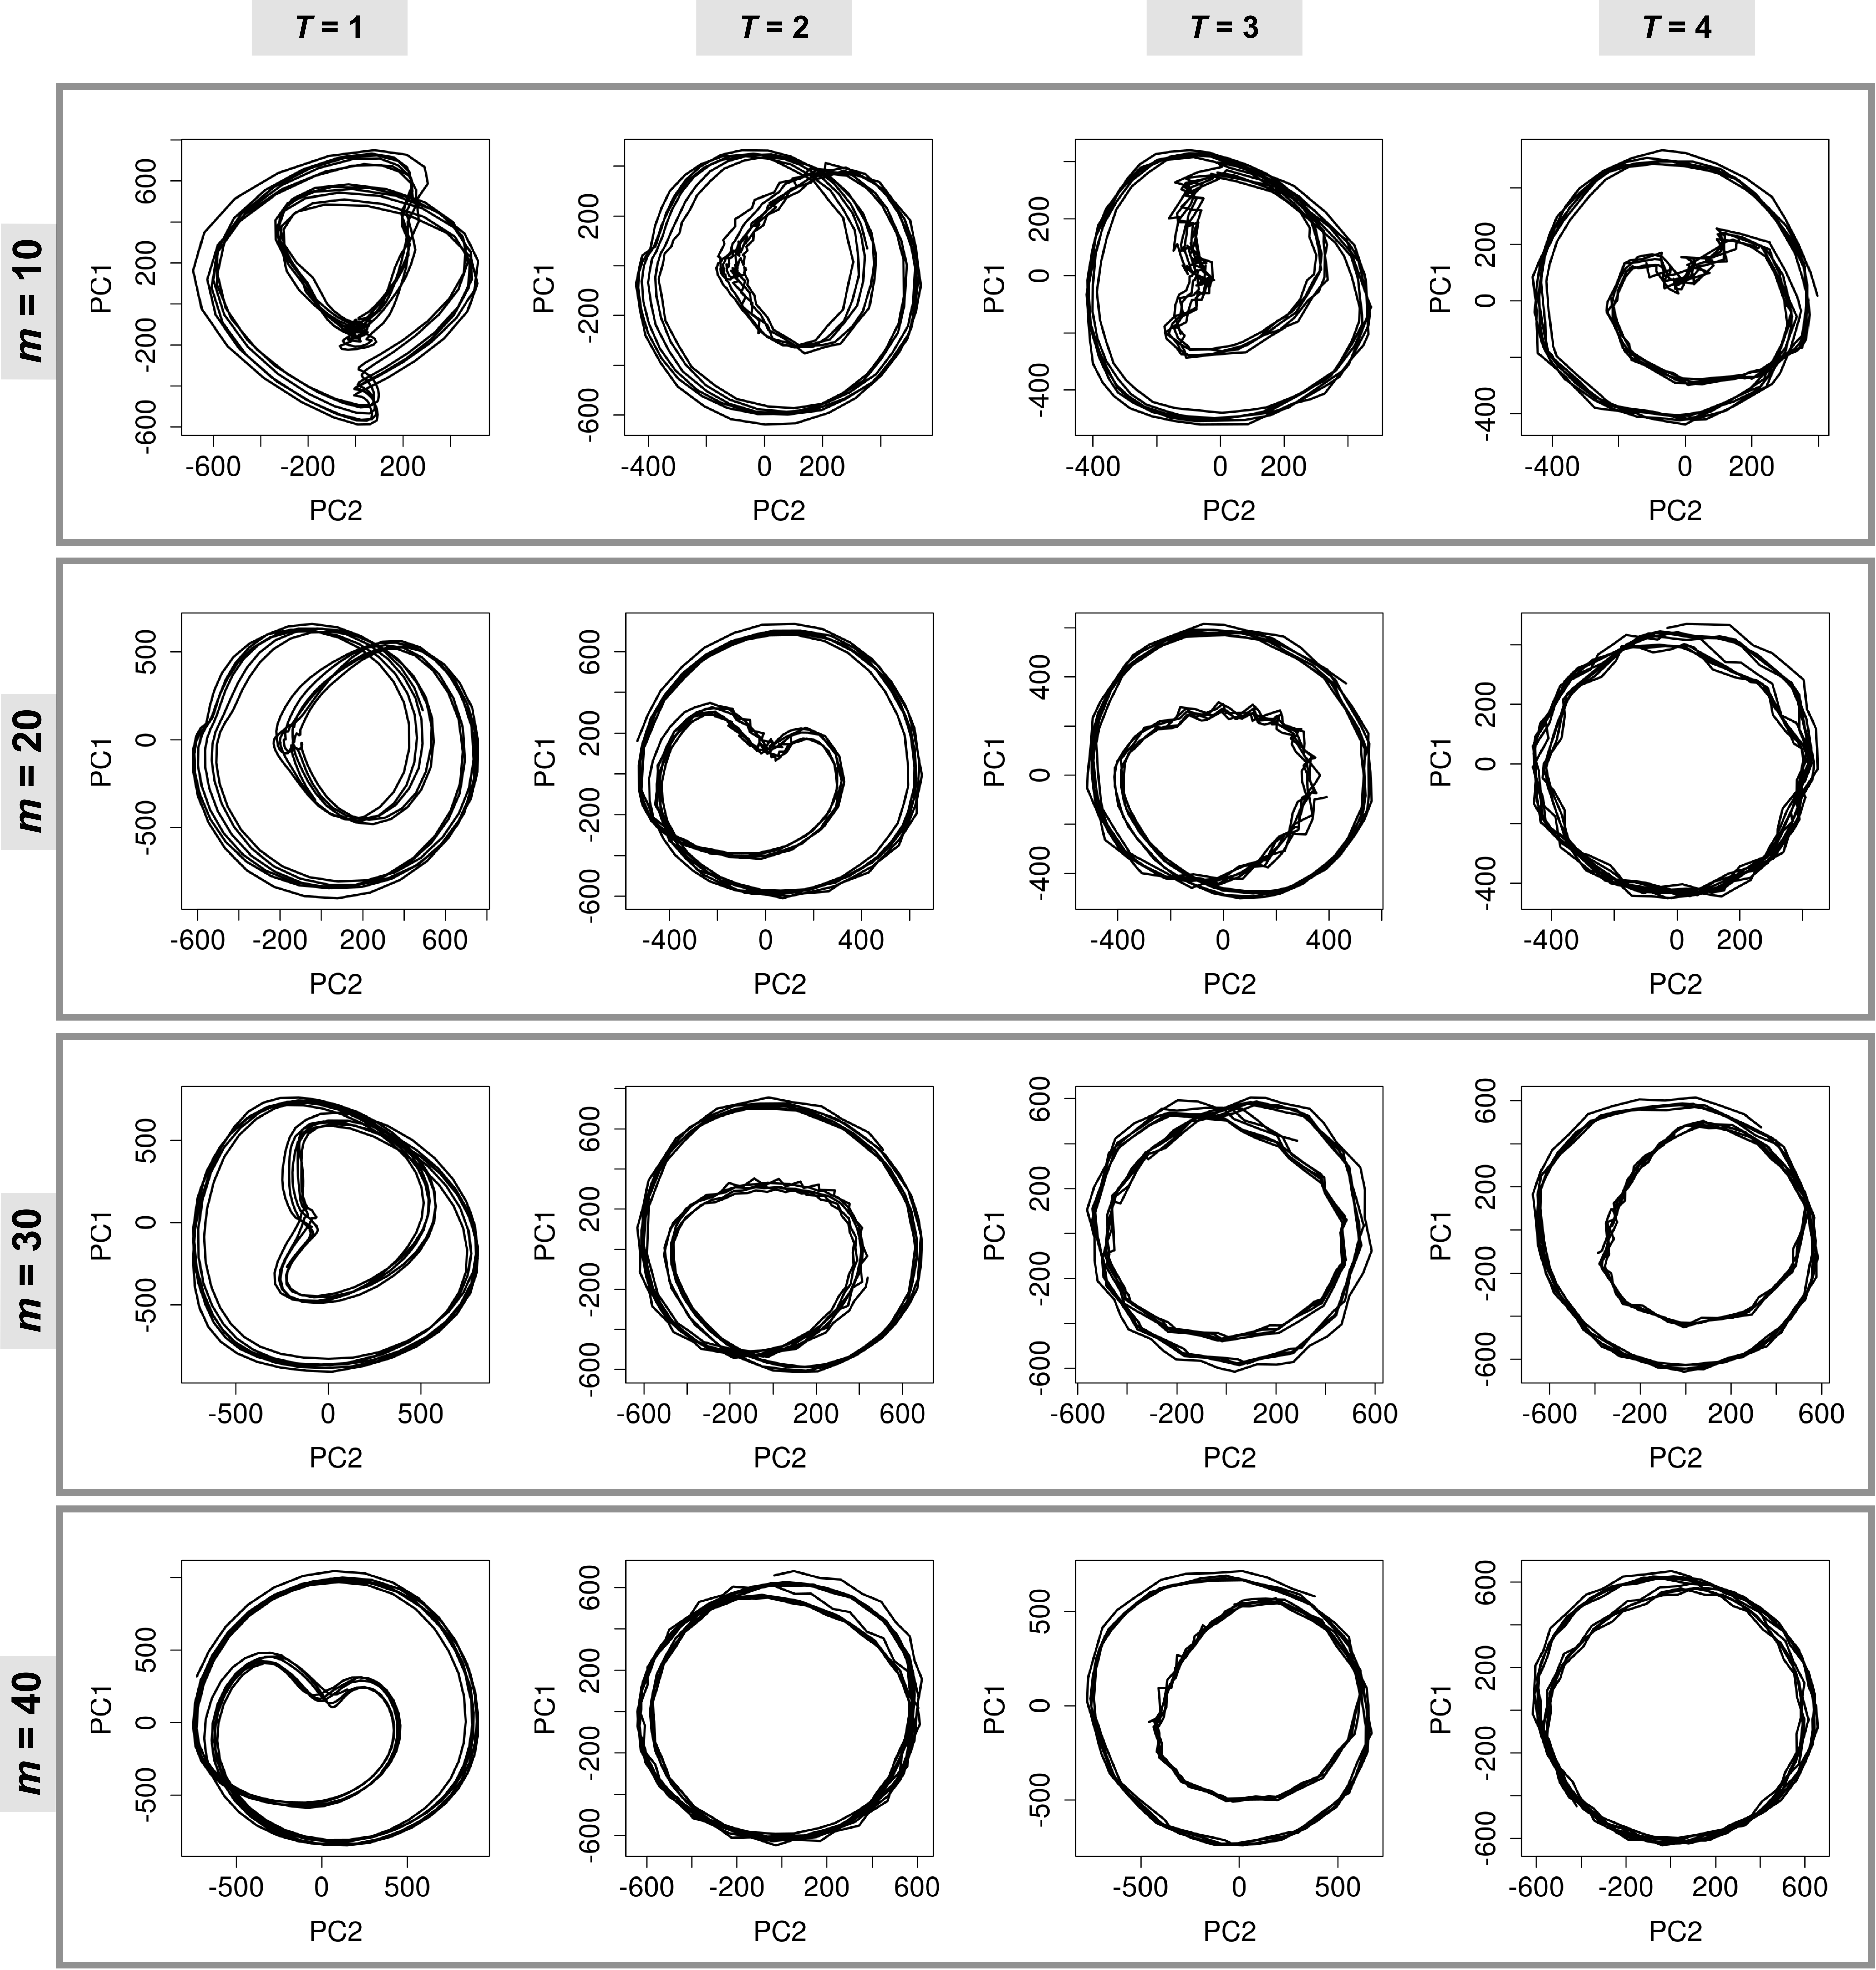
\includegraphics[width=0.45\textwidth]{takens}
\caption[PA]{2-D reconstructed state spaces with different embedded parameters ($m=10,20,30,40$ and $\tau= 1,2,3,4$)
for the same time-serie.}
\label{fig:takens_problem}
\end{figure}

\subsection{Skills assessment using only the PCA}
Hammerla et al. \cite{Hammerla2011} proposed the use of PCA with triaxial accelerometer sensor for skill assesment 
of the whisking activity. Prior to the PCA computation, raw data is whitened, i.e. each axis is normalised to have zero mean and unit variance.
Then the area between the cumulative energy percentage curve (CEP) and the diagonal is used as a metric for motor skill assesment.
We theferefore compute the cumulative energy using the triaxial whitening data in each sensor for step 1 and 2.
From Table~\ref{tab:table2} we can see that data from the magnetometer sensors has the highest variance 
of the $C_1 + C_2$ value for each of the users and steps with the exception of the intermedium participant in step 1. 
We therefore choose the magnetometer sensor for further analysis.
Figures ~\ref{fig:cumene} (a,e) present the CEP curves of raw data in which at least two out of three cumulative energy curves are overlaped. 

On the other hand, Figures ~\ref{fig:cumene} (b,d,c,f,g,h) illustrate the CEP curves using the time-delay embedded matrix as a different approach;
however, almost all the curves are overlaped.
It is therefore hard to establish significative differences among the curves to distinguish differences among expert, intermediate and 
non-dancers in each of the sensors.
\begin{figure*}[!t]
\centering    
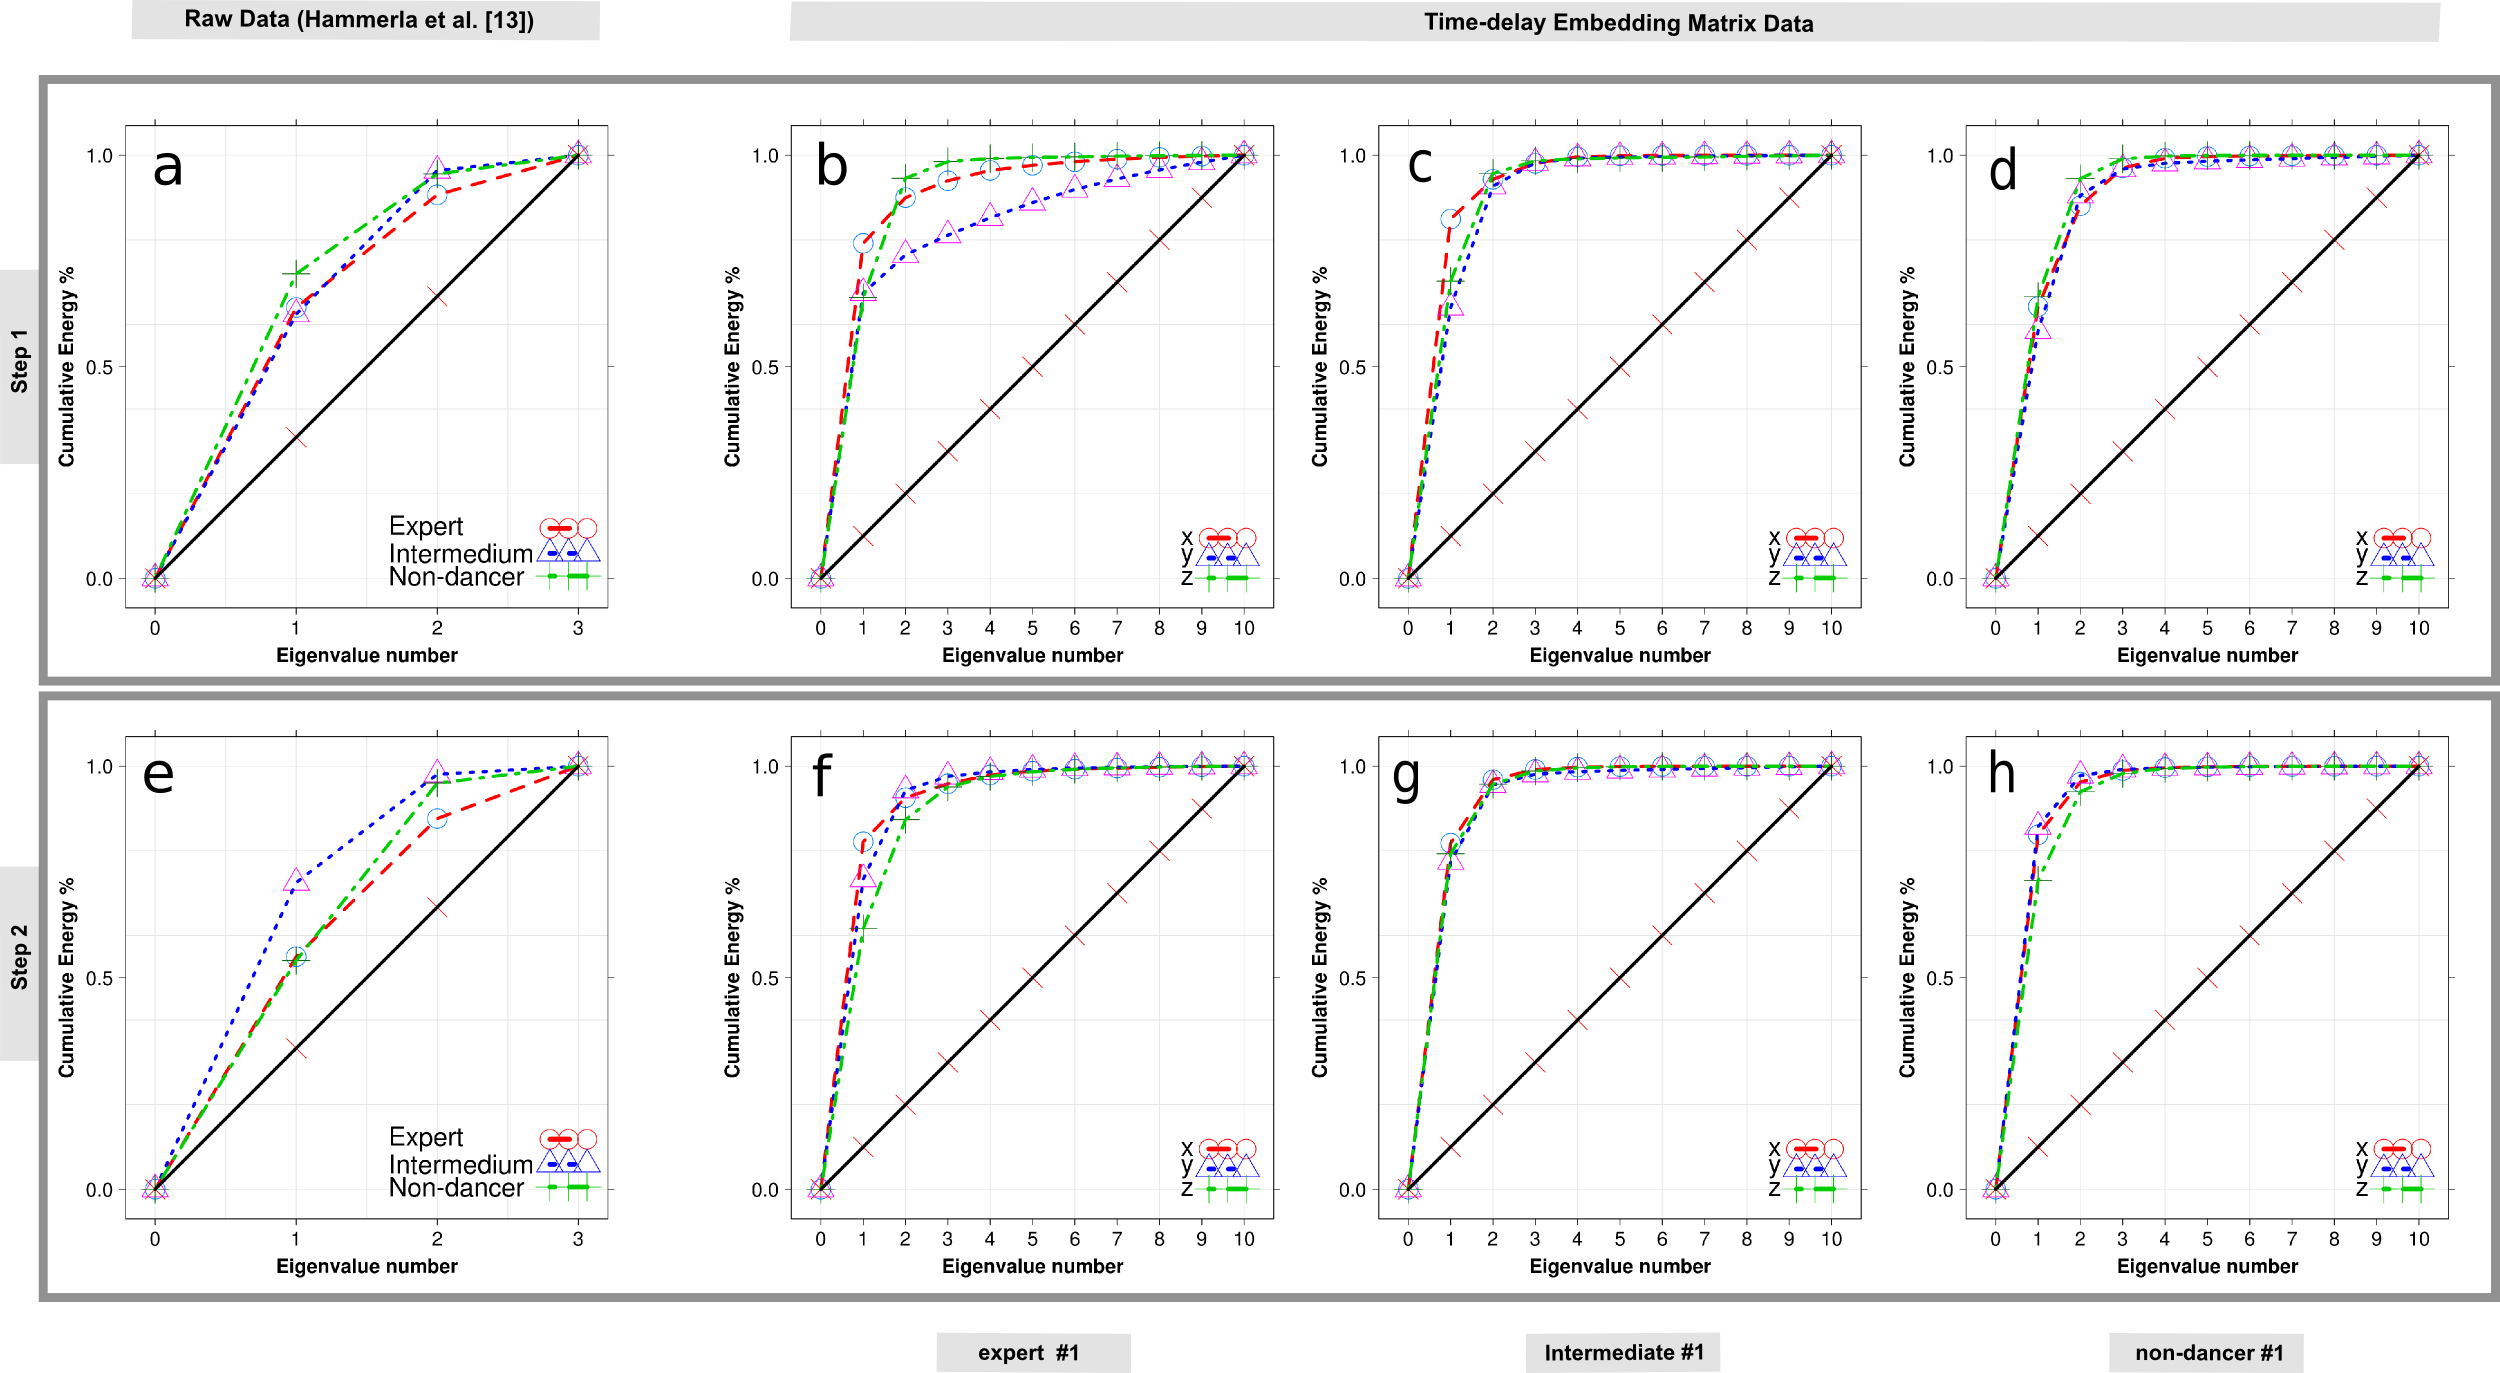
\includegraphics[width=1.0\textwidth]{cumulative_energy_magdata_drawing}
%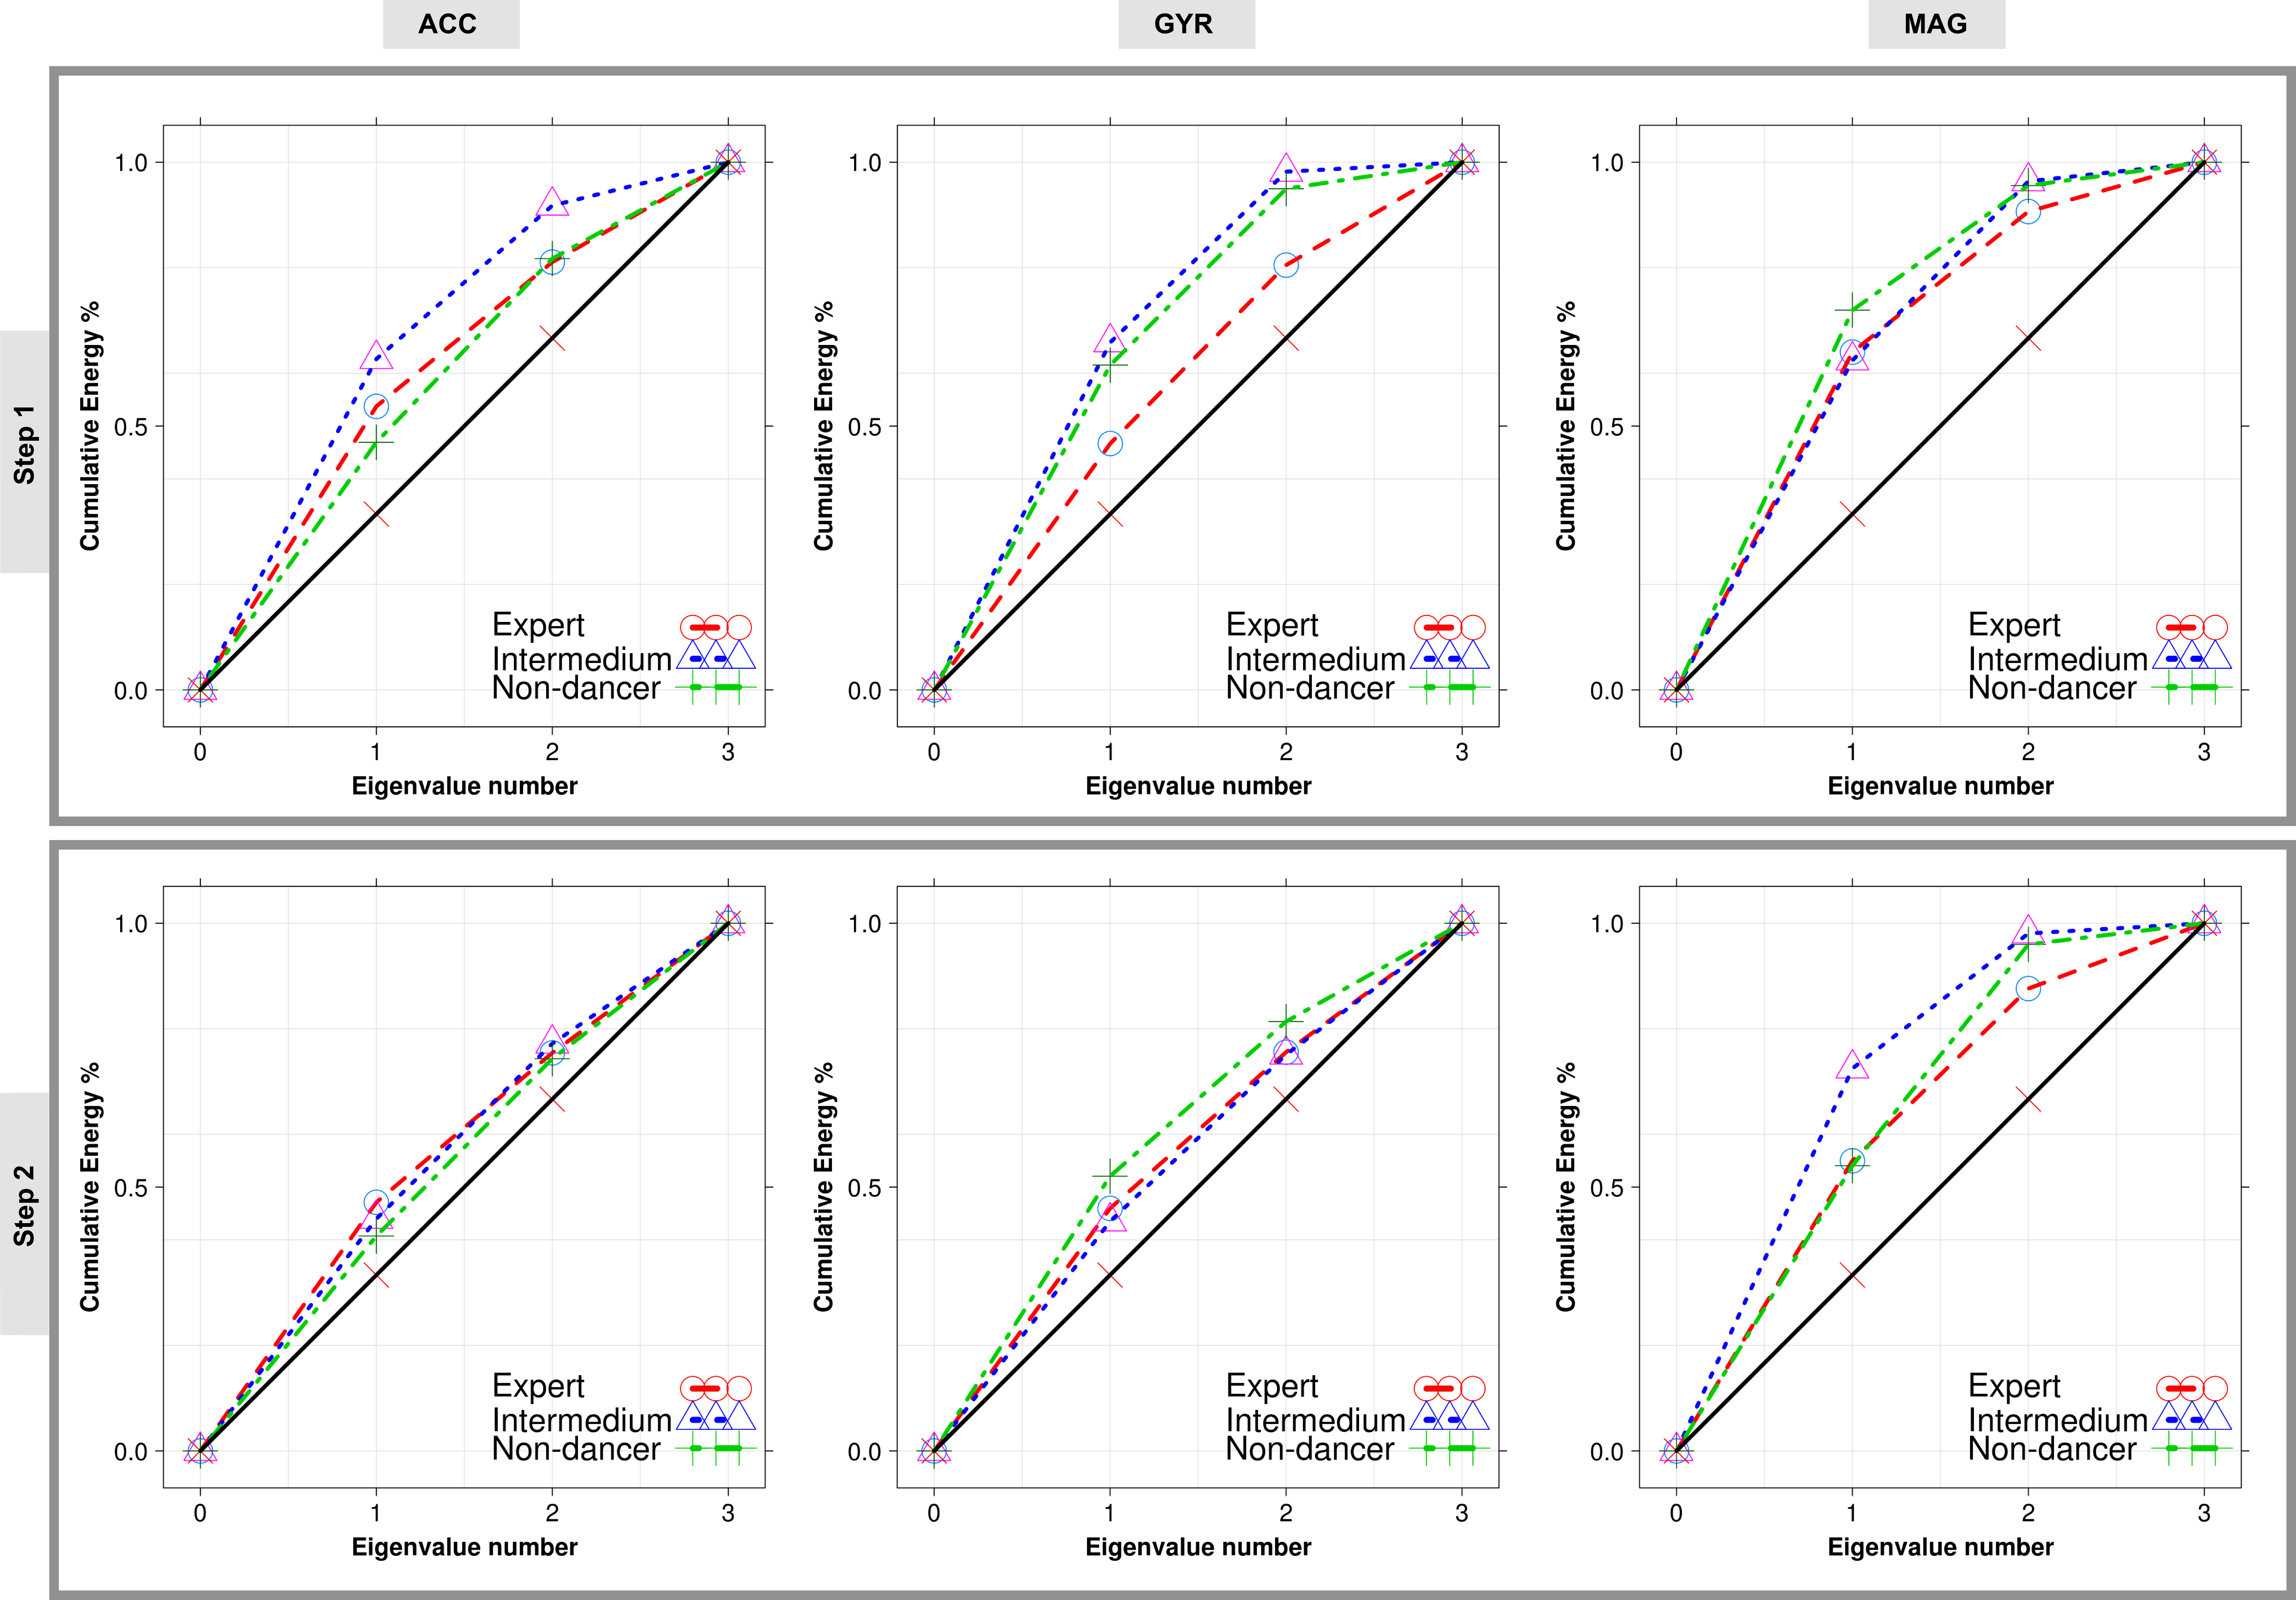
\includegraphics[width=1.0\textwidth]{cumulative_energy_whitening}
%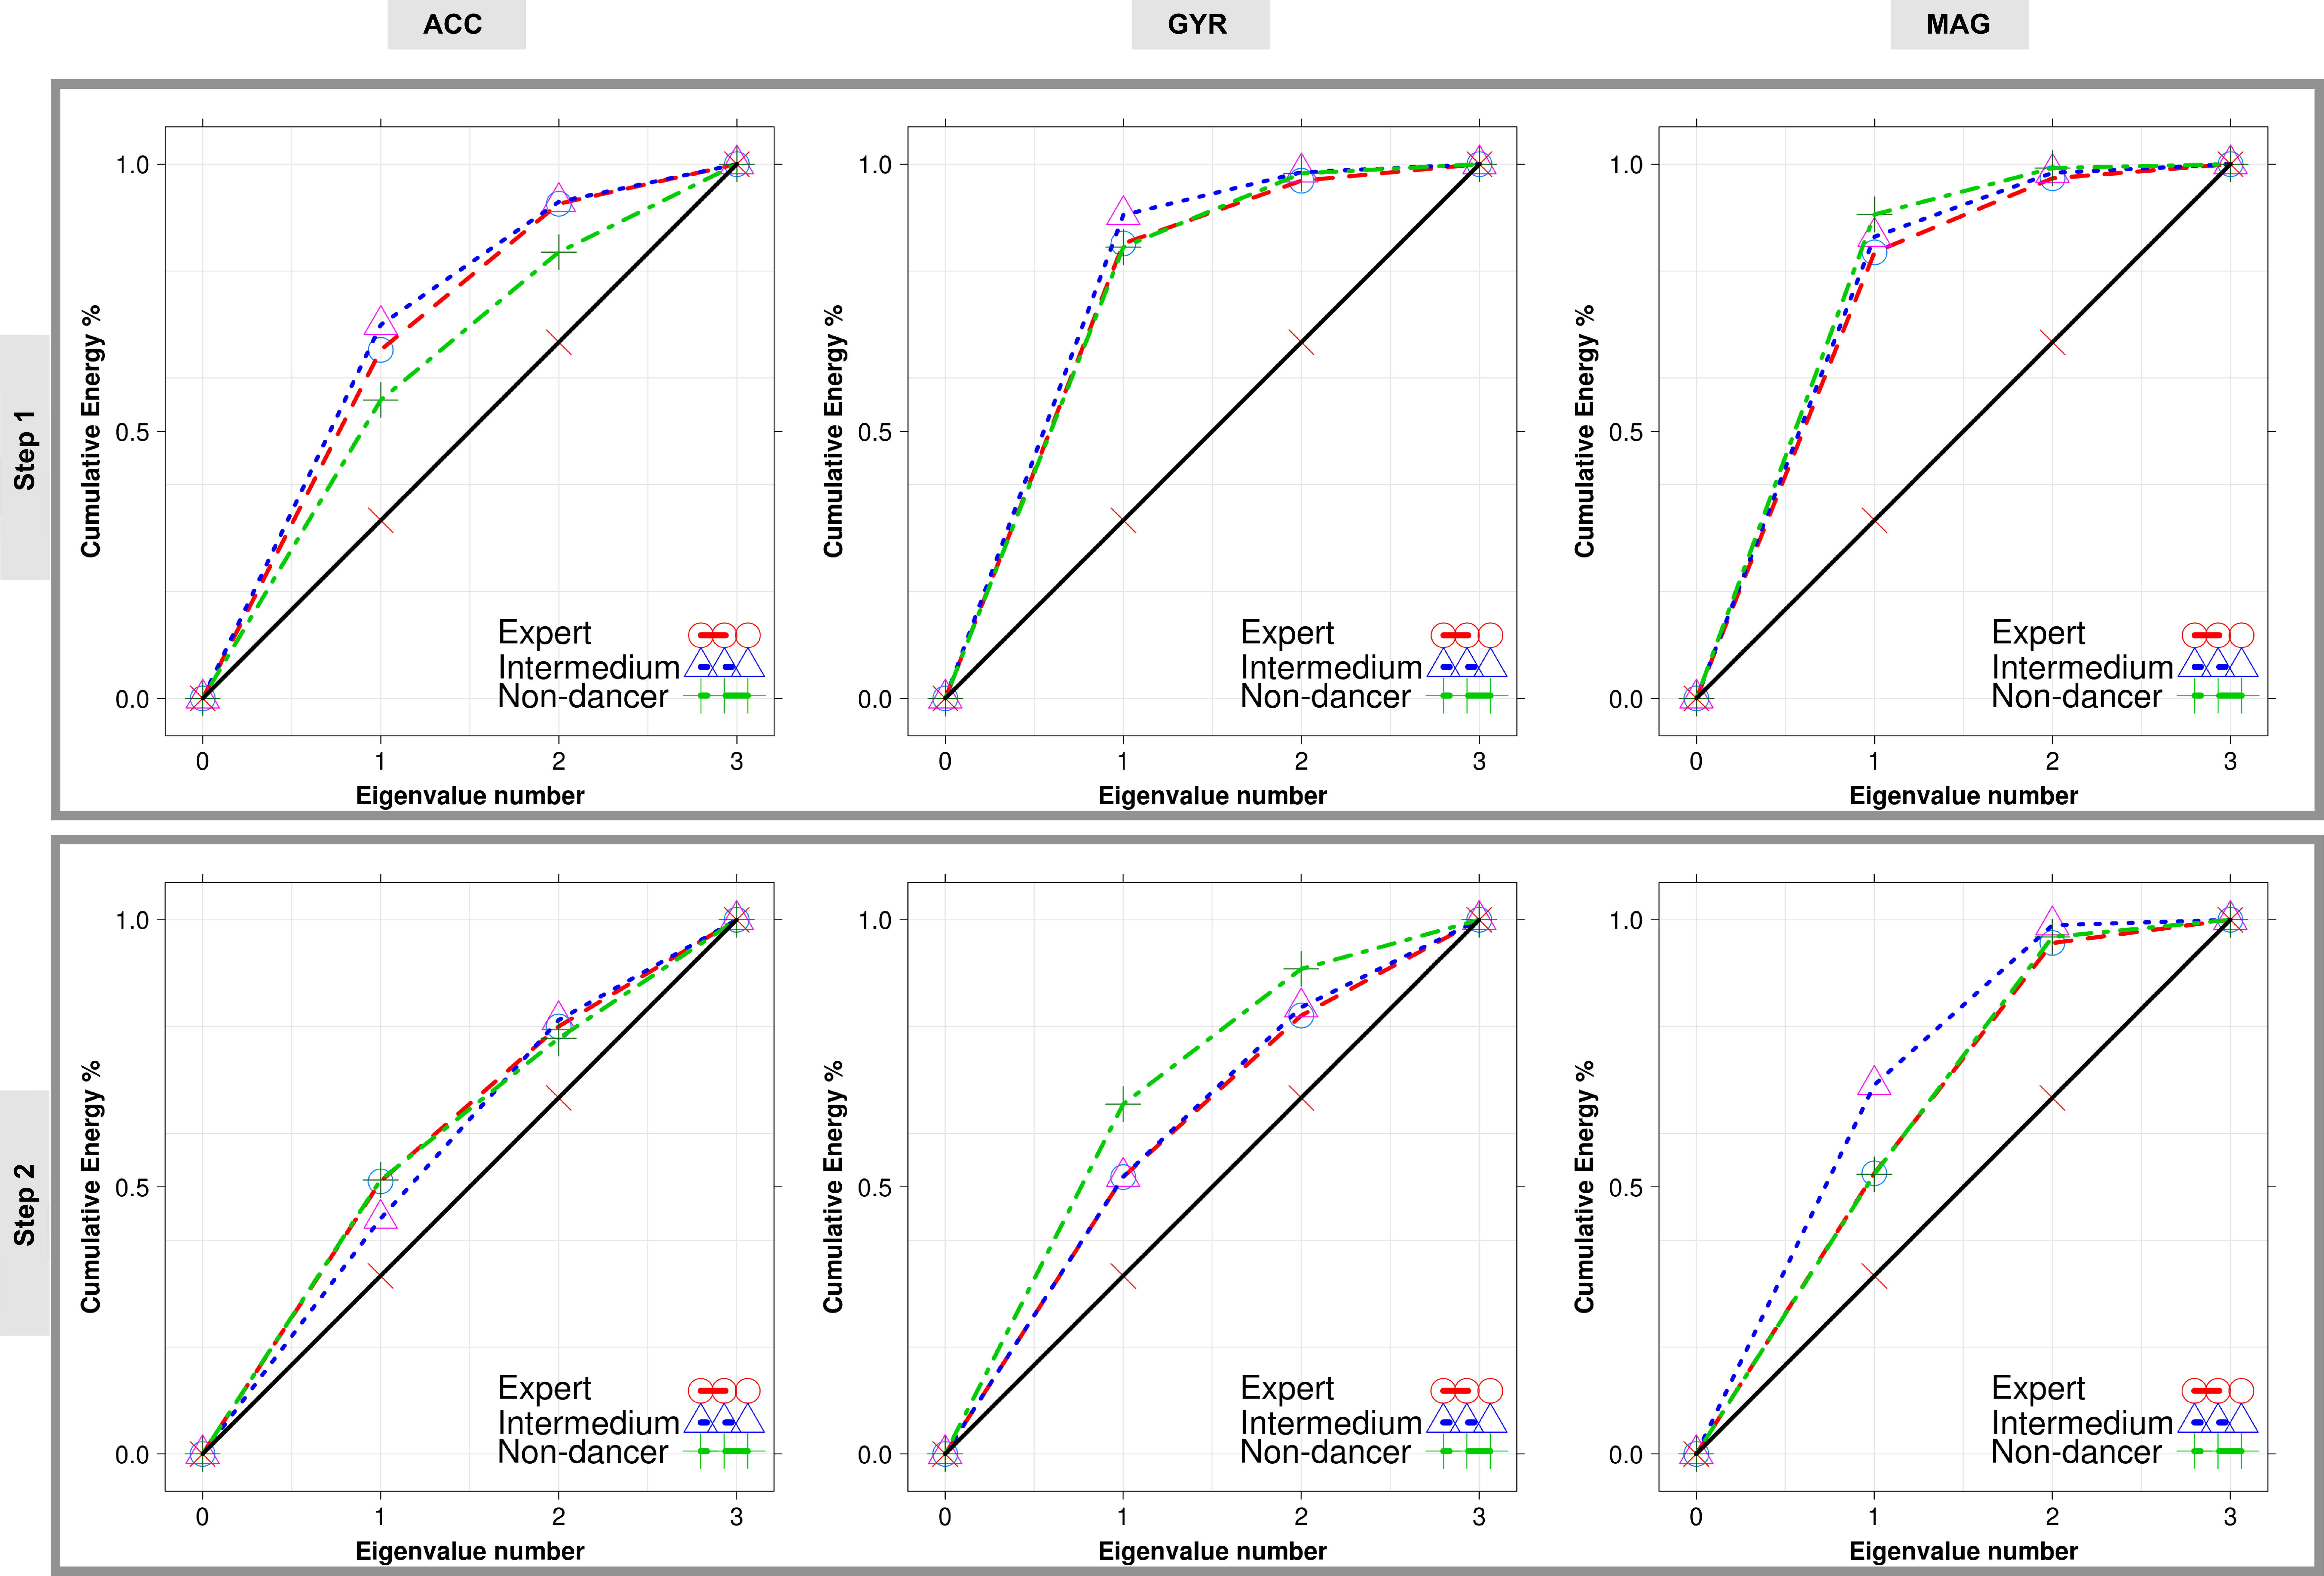
\includegraphics[width=1.0\textwidth]{cumulative_energy}
\caption[PA]{Cumulative energy percentage curves using the magnetometer sensor.
(a,e) curves are based on the triaxial raw data.
(b,d,c,f,g,h) curves are based on the time-delay embedded data for axis $x$, $y$ and $z$.
Curves are for expert, intermediate and non-dancer users for step 1 and step 2.}
\label{fig:cumene}
\end{figure*}
%However, there is no significant variation among the sensors's (ACC, GYR, and MAG) variance. 
% It is therefore proved that the cumulative energy is not well enought 
% as a metric for skills asessments in dance activities.
% 
% Neither the cumulative energy curves nor the 
% However, it is not possible to make any assumption of the level of dexterity by just considering the values of 
% the variations nor with the plot of the first two components as shown in Figure X.
% as shown in 
% 
% 
% Hammerla algorithm is not well replicable 
% since there are only three components for which the cummulative energy is computed
% which is the same as the percentage of variance .
\begin{table}
\tiny

  \centering
  
\begin{tabular}{l c c c c c c }
\toprule



& \multicolumn{6}{c}{Expert} \\
\cmidrule(r){2-7}

& \multicolumn{3}{c}{Step 1} & \multicolumn{3}{c}{Step 2}\\
\cmidrule(lr){2-4} \cmidrule(lr){5-7}

     & $C_1$ & $C_2$  & $C_1+C_2$  & $C_1$  & $C_2$  & $C_1+C_2$  \\
\midrule

$\boldsymbol{ACC}$ & 53.72 & 27.33 & 81.06 & 47.12 & 28.31 & 75.43 \\
$\boldsymbol{GYR}$ & 46.68 & 33.81 & 80.50 & 45.96 & 29.59 & 75.56 \\
$\boldsymbol{MAG}$ &64.00 & 26.64 & \cellcolor{blue!25}90.65 & 54.97 & 32.64 & \cellcolor{blue!25}87.62 \\


& \multicolumn{6}{c}{Intermedium} \\
\cmidrule(r){2-7}

& \multicolumn{3}{c}{Step 1} & \multicolumn{3}{c}{Step 2}\\
\cmidrule(lr){2-4} \cmidrule(lr){5-7}

     & $C_1$ & $C_2$  & $C_1+C_2$  & $C_1$  & $C_2$  & $C_1+C_2$  \\
\midrule
$\boldsymbol{ACC}$ & 62.70 & 29.07 & 91.77 & 43.98 & 33.21 & 77.19 \\
$\boldsymbol{GYR}$ & 65.86 & 32.33 & \cellcolor{blue!25}98.19 & 43.49 & 31.61 & 75.11 \\
$\boldsymbol{MAG}$ & 62.44 & 33.93 & 96.37 & 72.48 & 25.58 & \cellcolor{blue!25}98.07 \\


& \multicolumn{6}{c}{Non-dancer} \\
\cmidrule(r){2-7}

& \multicolumn{3}{c}{Step 1} & \multicolumn{3}{c}{Step 2}\\
\cmidrule(lr){2-4} \cmidrule(lr){5-7}

     & $C_1$ & $C_2$  & $C_1+C_2$  & $C_1$  & $C_2$  & $C_1+C_2$  \\
\midrule
$\boldsymbol{ACC}$ & 46.91 & 34.81 & 81.73 & 40.72 & 33.60 & 74.32 \\
$\boldsymbol{GYR}$ & 61.55 & 33.41 & 94.97 & 52.06 & 29.30 & 81.36 \\
$\boldsymbol{MAG}$ & 71.96 & 23.60 & \cellcolor{blue!25}95.57 & 54.06 & 41.93 & \cellcolor{blue!25}95.99 \\

\bottomrule
\end{tabular}

  \caption{Percentages of variances of the first two PCA components and its addition
      %($C_1$, $C_2$, and $C_1 + C_2$)
       from triaxial accelerometer (ACC), gyroscope (GYR), and magnetometer (MAG) sensors.
  Colored cells represent the maxium percentange of variation of the fist two PCA components.}
  \label{tab:table2}
\end{table}



\section{RESULTS}
Figure ~\ref{fig:skills} illustrates the 2-D reconstructed state space for the 
non-dancer, intermediate and expert dancers which visually help us to distinguish different levels of skills. 
\begin{figure}[htbp!] 
  \centering    
  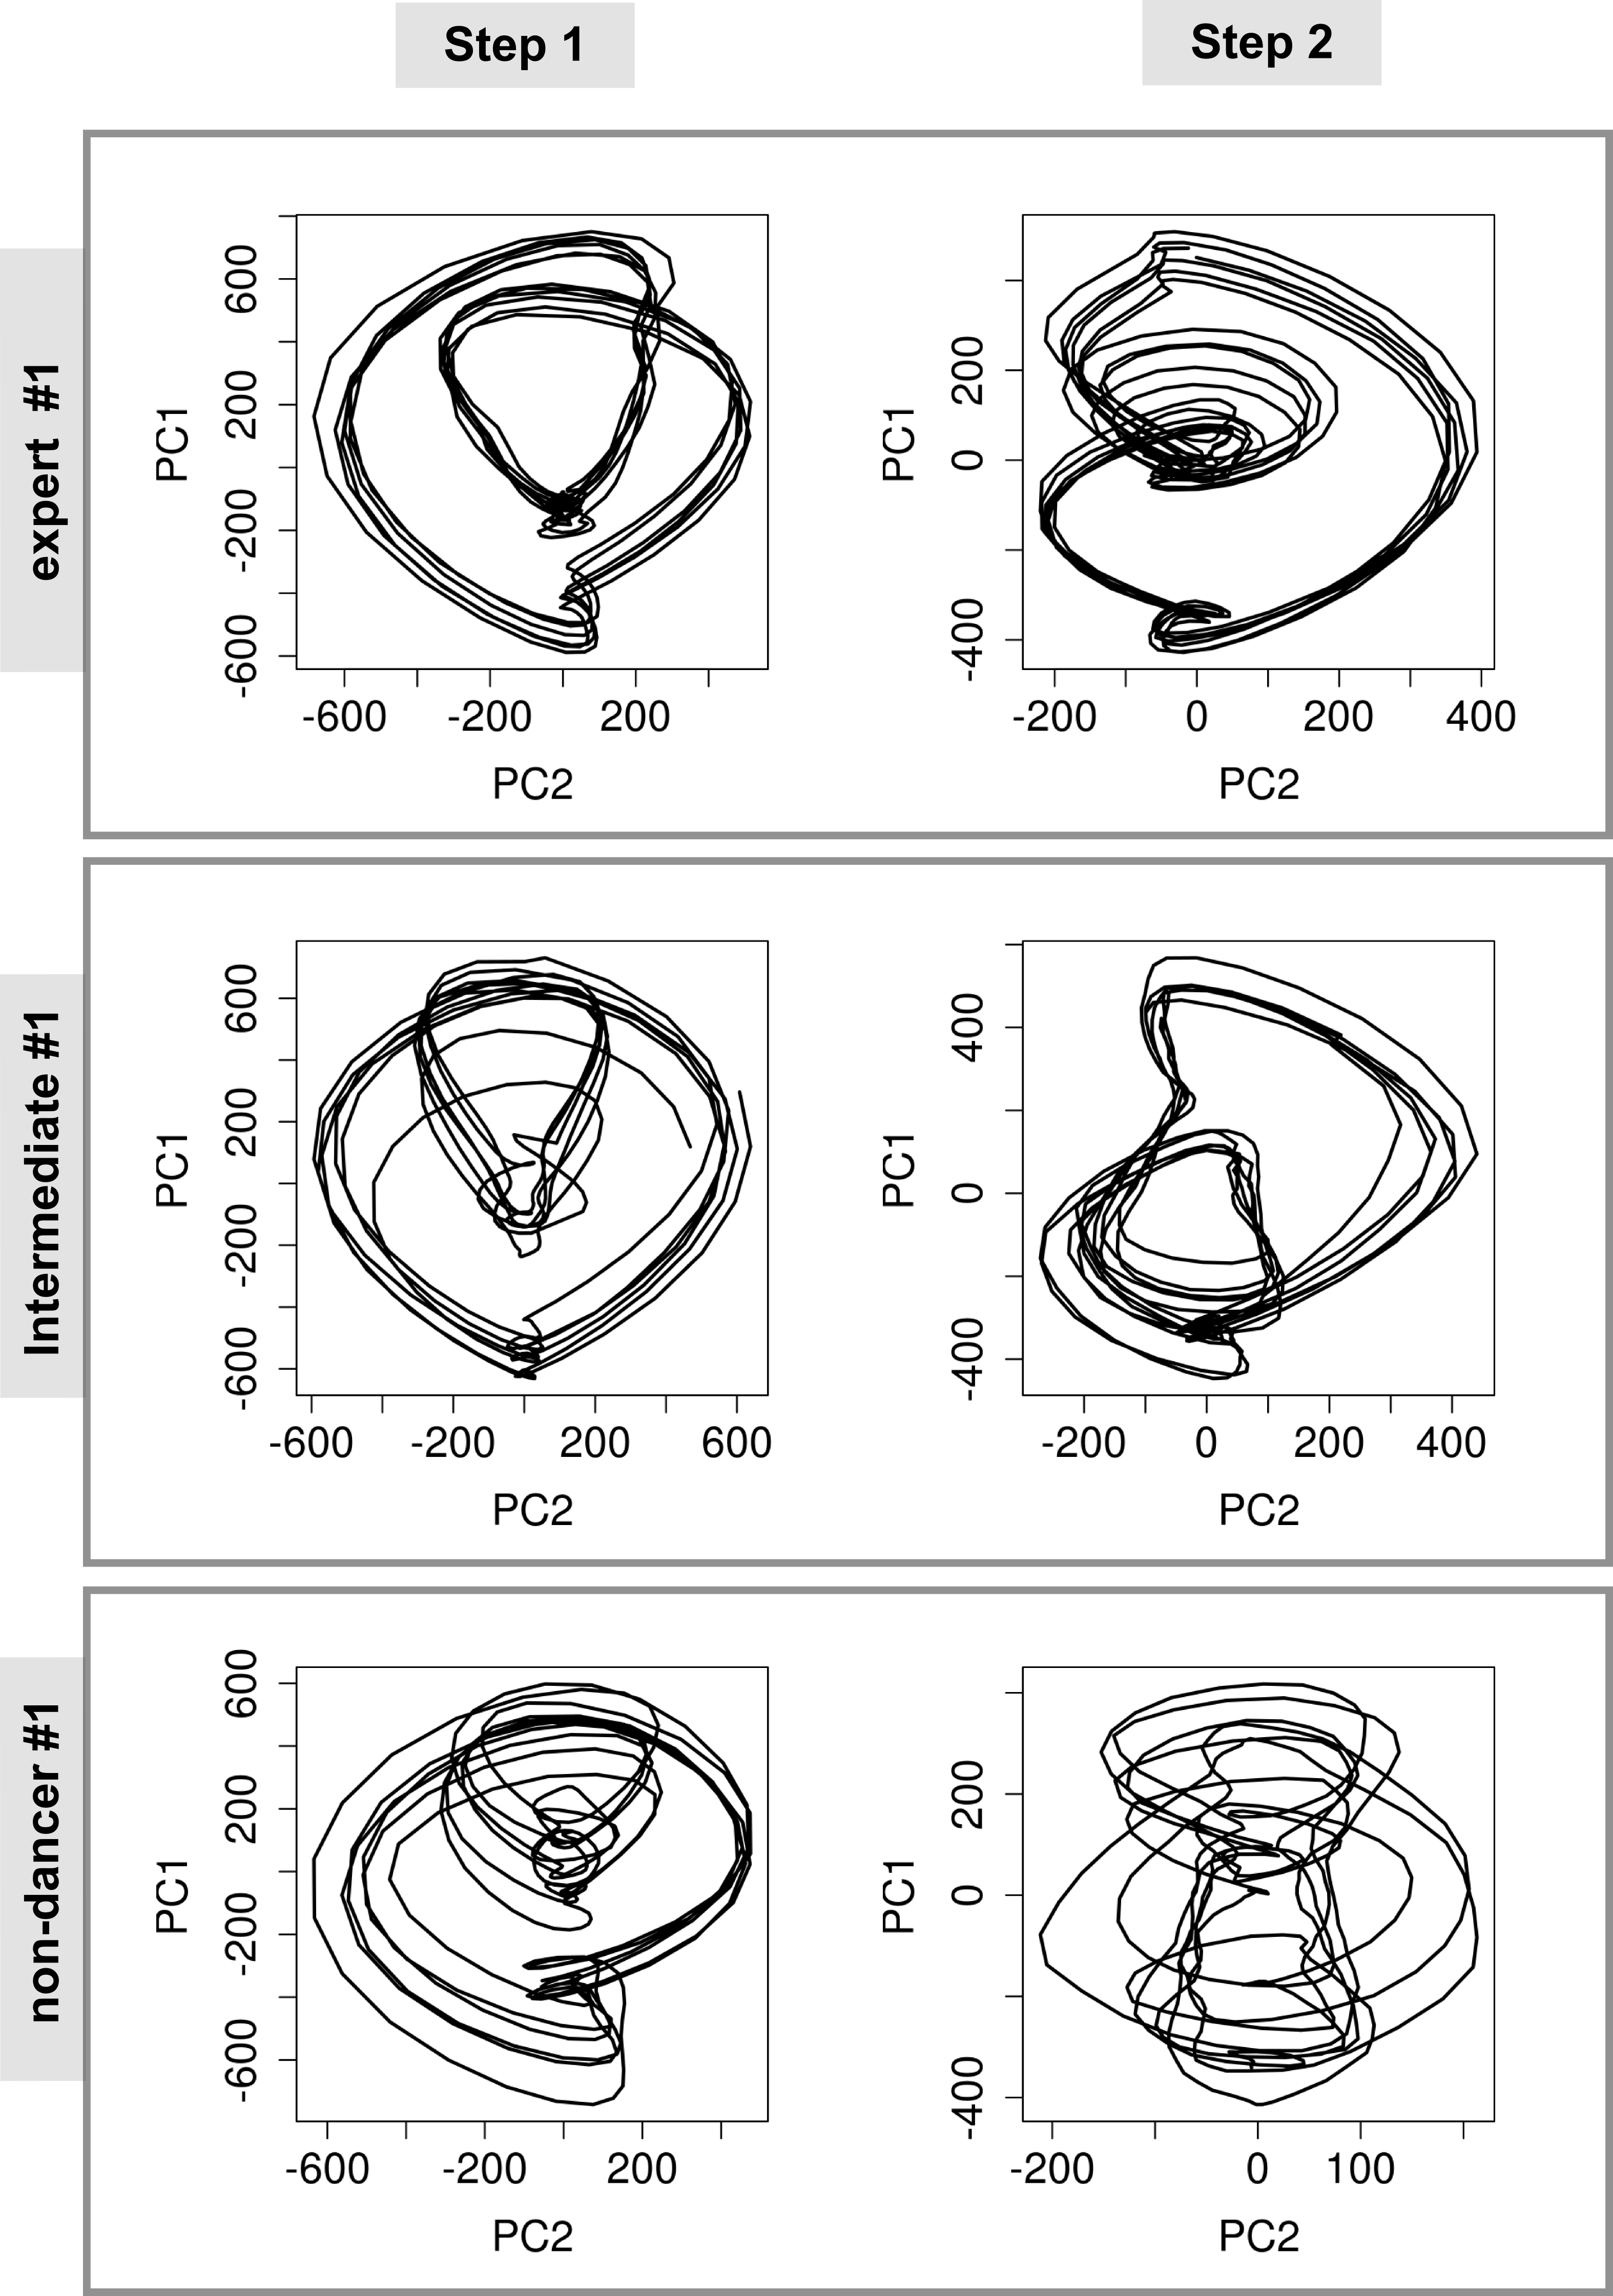
\includegraphics[width=0.45\textwidth]{skills}
  \caption[PA]{2-D reconstructed state spaces for the expert, intermediate and 
  non-dancer participants for step 1 ($m_z$ data) and step 2 ($m_y$ data). 
  First two component of the PCA for with embedding parameters ($m = 10$ and $\tau = 1$).}
  \label{fig:skills}
  \end{figure}
It is immediately noticeable that the shape of the state space for each level (novice, intermediate, expert) 
appear visually similar across step 1.  
As the participants are meant to be performing the same action, this similarity is to be expected.  
However, the state spaces also show a tighter and less varied pattern for the expert than for the other skill levels.  
This suggests that the expert is producing more repeatable, more consistent actions than the other skill levels.  
While this is to be expected, the reconstructed state spaces provide interesting illustrations of this phenomenon.  
For step 2, on the other hand, (which was a more complicated sequence of movements),
one can see a marked contrast across skill levels.  
Again, the expert is showing a consistent and repeatable action.  
The intermediate participant is showing a consistent action but this is different to that of the expert, 
and the novice is showing a pattern which appears disjointed and noisy.  
Indeed, for the novice dancer, the state space reconstruction of step 2 seems to have more in common 
with their state space for step 1 than it does with the other dancers performing step 2.  

\section{DISCUSSION}
Although the Takens' Theorem is still subject to the embedded parameters, 
the phase space representation applies a model of consistency to the data for skill assessment. 
The control of variability then becomes desirable because expert dancers are better able to moderate 
their actions in response to contextual demands in a way that produces a state space reconstruction 
that appears consistent.  The novice dancer, on the other hand, appears to been producing similar 
patterns of movement for both steps rather than attempting to fully engage with the requirements of step 2.  

While the results provide some indication of difference between levels of skill, the interpretation of 
the state space reconstructions remains qualitative.  While this is not unusual in the literature
which applies time-delay embedding to the analysis of human activity, further work is required to develop 
reliable and robust techniques to analyse these reconstructions.  
A promising line of enquiry would be to investigate the geometry of the state space reconstructions
which could be used to support comparison \cite{Sama2013} and also could aid in the computation of the minimal 
embedded parameters. 
 
The results in this paper are only from a single axis of a single sensor. 
One can see from the $E2(d)$ values that the accelerometer data is more noisy since its variance is 
more spreaded in the components of the PCA than that from the gyroscope and magnetometer.  
While this is most likely due to effects of gravity on the accelerometer 
(although the ADXL345 accelerometer used in the Razor offers simple gravity compensation), 
there interference with the signal can be further filtered and compensated.  
It would be interesting to determine how combinations of sensor data can be used to create similar 
state space reconstructions and this will be explored in the next phase of work. 
The magnetometer sensor in the z-axis for step 1 and the magnetometer sensor in the y-axis for step 2
have the highest variance which related to the determinism of the signals.

We demonstrated that Hammerla's method is not appropriable for dexterity assesment using 
raw data from the intertial sensors as well as the use of the time-delay embedded matrix data
since the cummulative energy percentage curves are hardly indistinguished from 
both the level of expertise and the type of step.

The aim of this work is to measure dexterity in dance from wearable IMUs. Data from the IMUs are presented
in a canonical basis that reflects the non-linear dynamics pf dance steps. On the basis to this analysis we can 
distinguish expert, intermediate amd beginner levels of dexterity for two dance steps.
% Future work, investifate the preservation of geometry \cite{Yap2014} 
% for the computation of the minimal embedded parameters.


\section{Acknowledgments}
The work reported in this paper is partly supported by a studentship from
National Council for Science and Technology, CONACyT, Mexico.



% Balancing columns in a ref list is a bit of a pain because you
% either use a hack like flushend or balance, or manually insert
% a column break.  http://www.tex.ac.uk/cgi-bin/texfaq2html?label=balance
% multicols doesn't work because we're already in two-column mode,
% and flushend isn't awesome, so I choose balance.  See this
% for more info: http://cs.brown.edu/system/software/latex/doc/balance.pdf
%
% Note that in a perfect world balance wants to be in the first
% column of the last page.
%
% If balance doesn't work for you, you can remove that and
% hard-code a column break into the bbl file right before you
% submit:
%
% http://stackoverflow.com/questions/2149854/how-to-manually-equalize-columns-
% in-an-ieee-paper-if-using-bibtex
%
% Or, just remove \balance and give up on balancing the last page.
%
\balance



\bibliographystyle{acm-sigchi}
\bibliography{references}
\end{document}
